\documentclass{article}

\usepackage[english]{babel}
\usepackage[letterpaper,top=2cm,bottom=2cm,left=3cm,right=3cm,marginparwidth=1.75cm]{geometry}

\usepackage{amsmath}
\usepackage{graphicx}
\usepackage{booktabs}
\usepackage{subcaption}
\usepackage[colorlinks=true, allcolors=blue]{hyperref}

\graphicspath{{plots/}}

\title{Canon Layer Exploration Report}
\author{Kirill Zemlianskii}

\begin{document}
\maketitle

\begin{abstract}
  abstract
\end{abstract}

% ---------------------------------------------------------------------------
\section{Data: Synthetic Benchmarks}
\label{sec:data}
% ---------------------------------------------------------------------------

\subsection{Task Descriptions}
\label{sec:data:tasks}

\paragraph{Depo.}
Depo~\cite{allen_zhu_physics4} is a synthetic reasoning benchmark that tests multi-hop
knowledge retrieval. Each training instance encodes $n$ directed edges of a circular
permutation followed by one or more queries. A query specifies a start node $q$ and a hop
distance $k$; the model must predict the $k$-th successor without intermediate chain-of-thought
steps. Formally, each sequence has the form
\[
  \langle\text{bos}\rangle\; x_1\,y_1\;\cdots\; x_n\,y_n\;
  \langle\text{query}_k\rangle\; q\; a\; \langle\text{eos}\rangle,
\]
where $y_i = f^k(x_i)$ for the ground-truth permutation $f$. The model is trained only on
the answer tokens $a$. The benchmark admits two variants: Depo1 uses 1--2-token nodes
(base vocabulary 50, $K{=}8$) and Depo2 uses 5--7-token nodes (base vocabulary 3,
$K{=}16$).

\paragraph{Brevo.}
Brevo~\cite{allen_zhu_physics4} evaluates \emph{reasoning breadth}: the ability to
process multiple dependencies simultaneously. Each instance encodes a
directed acyclic graph (DAG) of at most $N$ nodes, each of in-degree at most 4, followed
by a query vertex $q$:
\[
  \langle\text{bos}\rangle\; x_1\,y_1\;\cdots\; x_m\,y_m\;
  \langle\text{query}\rangle\; q\;
  \langle\text{ans}\rangle\; a_1\,a_2\,\cdots\,a_p\; \langle\text{eos}\rangle.
\]
The model must output all vertices recursively reachable from $q$, sorted in topological
order from the leaves inward. Because valid topological orderings are non-unique, the
model must mentally compute the \emph{full} topological order of the DAG before
generating the first answer token, making this a demanding breadth-first reasoning
task~\cite{allen_zhu_physics4}. Two variants are used: Brevo1 (single-token vertex
names, $N \in \{70, 90, 110\}$, sequences up to 1024 tokens) and Brevo2 (2--4-token
vertex names, $N \in \{30, 40, 50\}$, sequences up to 1536 tokens).

\subsection{Stability Across Seeds}
\label{sec:data:stability}

A central question is whether these benchmarks produce reliable, reproducible training
curves. We trained the same model architecture multiple times with different random seeds
and compared the resulting loss trajectories.

\paragraph{Text modeling is stable.}
As a reference, Figure~\ref{fig:text_stability} shows two Llama and two Canon seeds on
the standard FineWeb-Edu text modeling task. The curves are nearly indistinguishable
within each model class, confirming that the observed variance on synthetic tasks is
not caused by general optimizer noise.

\begin{figure}[h]
  \centering
  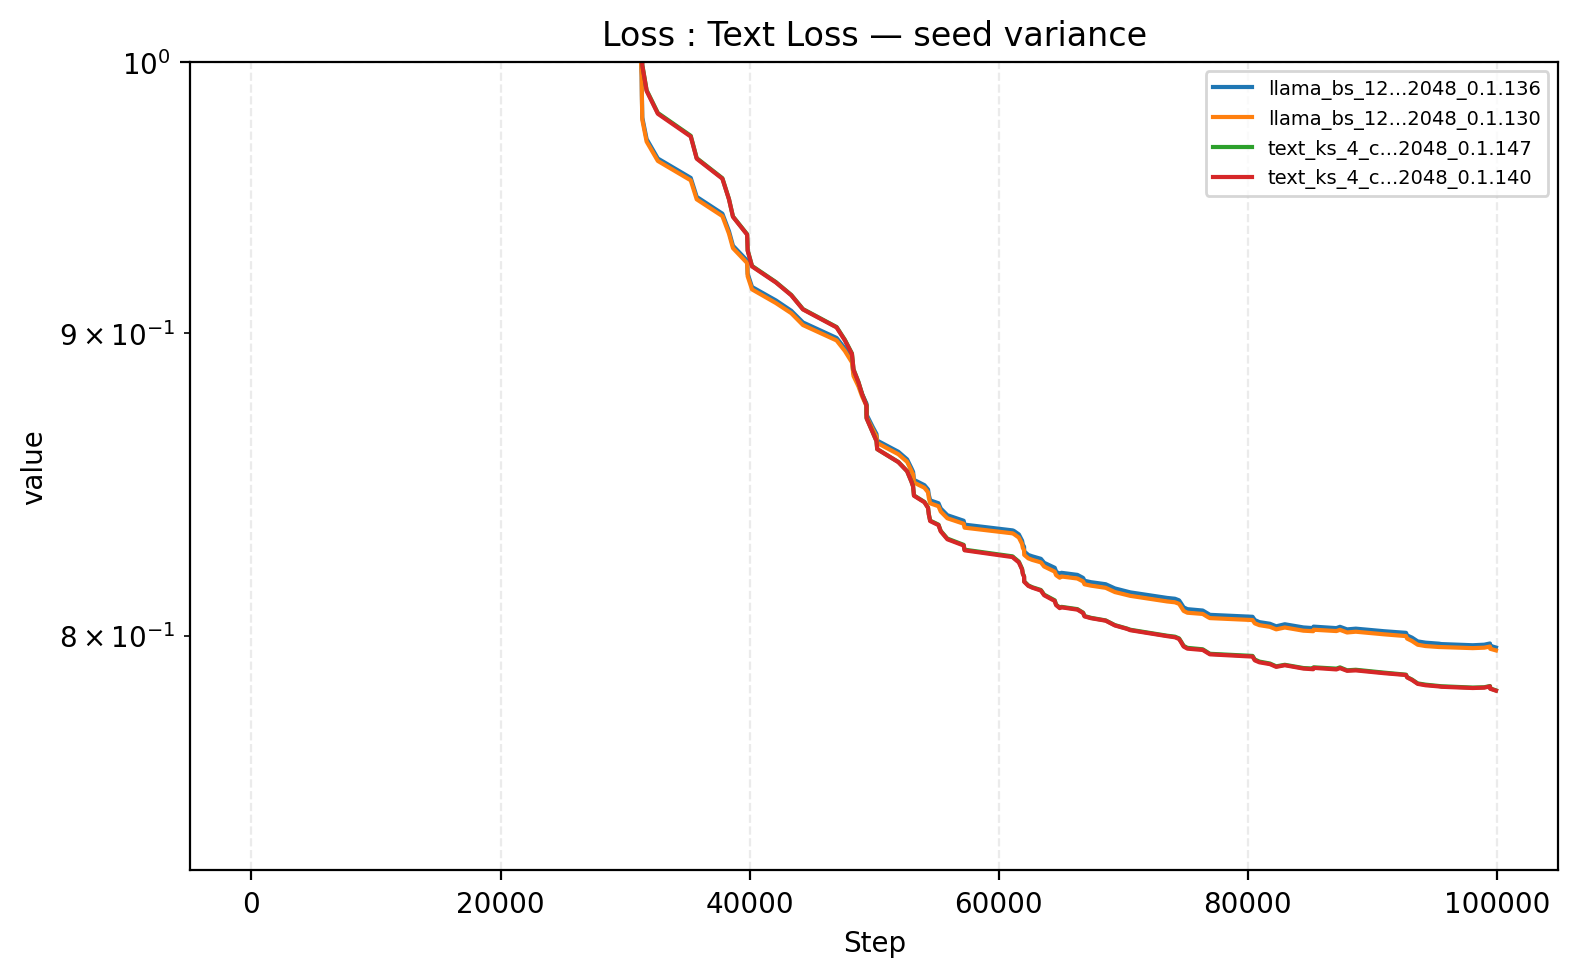
\includegraphics[width=0.7\linewidth]{march09_stability_text_loss.png}
  \caption{Training loss for two Llama seeds and two Canon seeds on text modeling.
    Curves within each model class overlap, demonstrating negligible seed-to-seed variance.}
  \label{fig:text_stability}
\end{figure}

\paragraph{Depo exhibits large seed-to-seed variance.}
Figures~\ref{fig:depo_8l} and~\ref{fig:depo_12l} show Depo training for an 8-layer/512-dim
model and a 12-layer/768-dim Canon model respectively.

\begin{figure}[h]
  \centering
  \begin{subfigure}[b]{0.48\linewidth}
    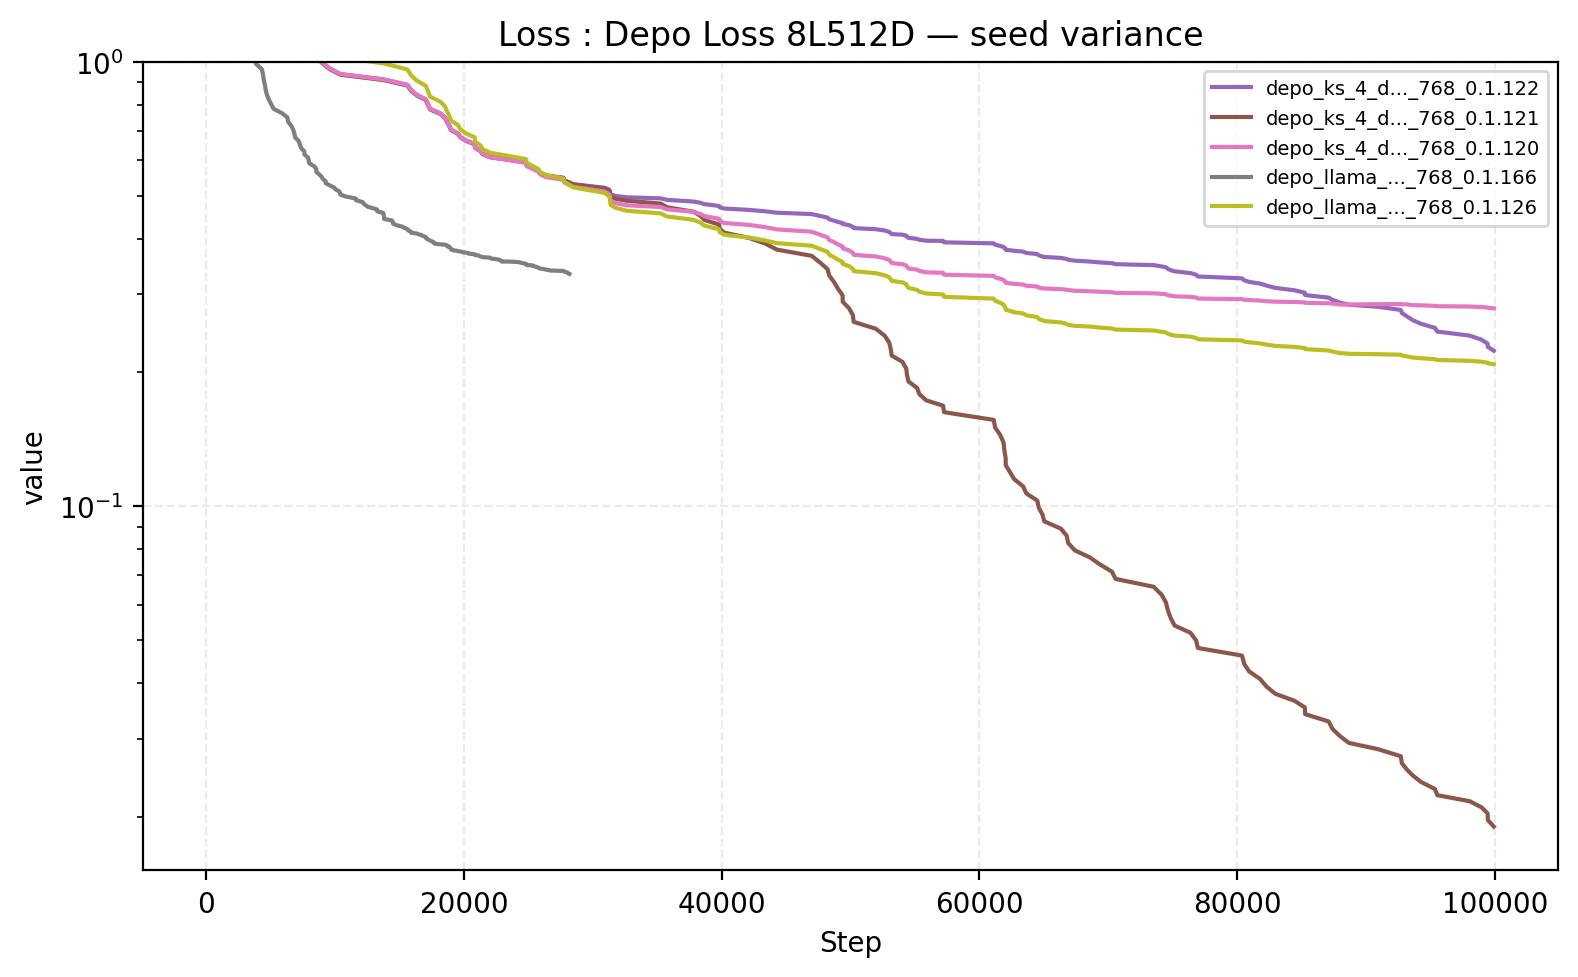
\includegraphics[width=\linewidth]{march09_stability_depo_8l512d_loss.png}
    \caption{8L/512D — Llama and Canon seeds.}
    \label{fig:depo_8l}
  \end{subfigure}
  \hfill
  \begin{subfigure}[b]{0.48\linewidth}
    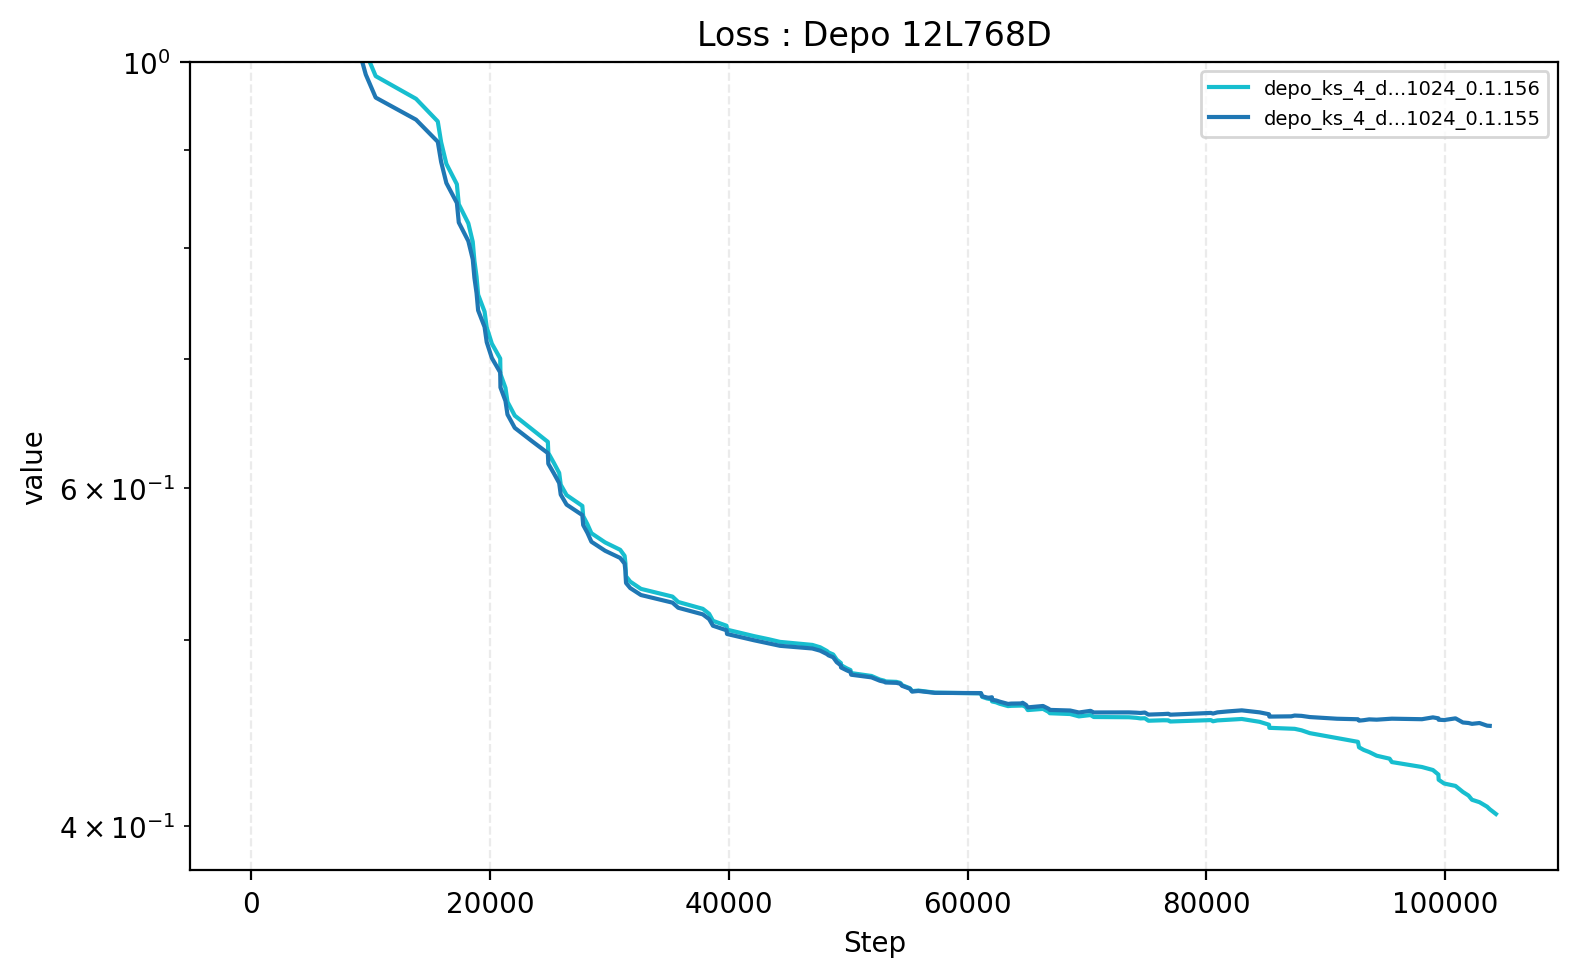
\includegraphics[width=\linewidth]{march09_stability_depo_12l768d_loss.png}
    \caption{12L/768D — two Canon seeds.}
    \label{fig:depo_12l}
  \end{subfigure}
  \caption{Depo training loss across seeds. In the 8L/512D setting one Llama seed
    converges dramatically faster than all other runs. In the 12L/768D setting one
    Canon seed stagnates throughout while the other undergoes a sudden grokking event,
    dropping sharply after many steps of little progress.}
  \label{fig:depo_stability}
\end{figure}

The 8-layer model training shows that the benchmark outcome flip depending
solely on random initialization. The 12-layer result illustrates a \emph{grokking}
regime~\cite{power2022grokking}: one seed never solves the task while the other
eventually solves it after a prolonged plateau. Figure~\ref{fig:depo_all_tokens} shows
the same effect when loss is computed over all tokens rather than answer tokens only.

\begin{figure}[h]
  \centering
  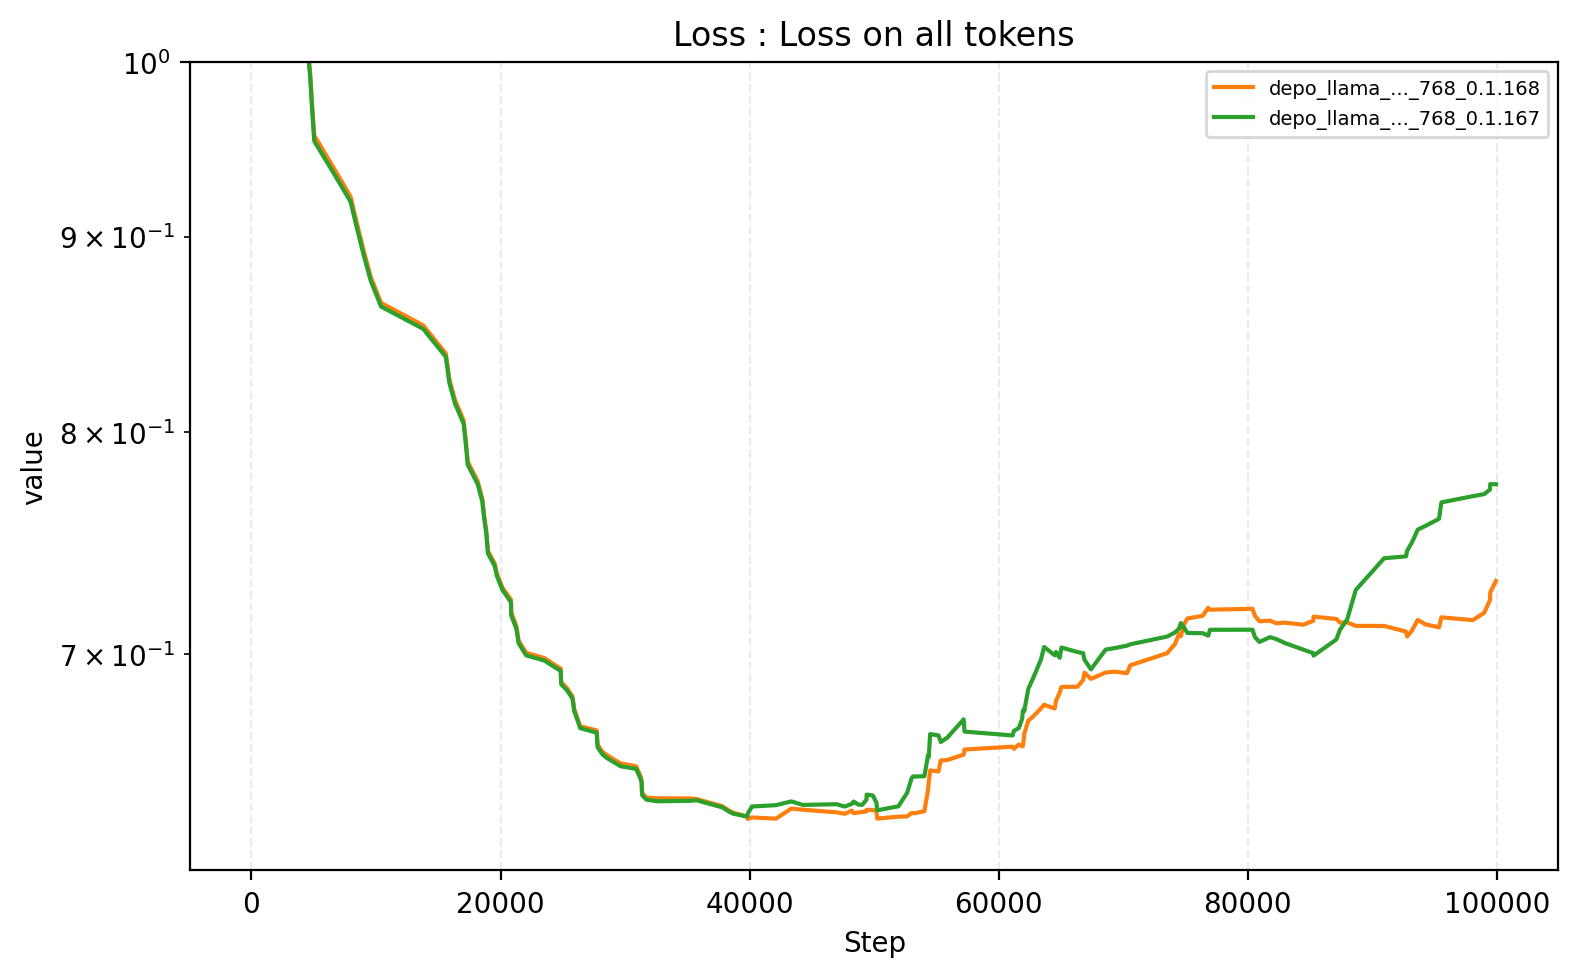
\includegraphics[width=0.7\linewidth]{march09_stability_depo_all_tokens_loss.png}
  \caption{Depo loss computed on all tokens (including context), confirming the same
    high variance observed on answer tokens alone.}
  \label{fig:depo_all_tokens}
\end{figure}

\paragraph{Brevo exhibits the same instability.}
Figure~\ref{fig:brevo} shows three Brevo seeds for a 110-node single-node configuration.
All three runs diverge from one another, with no sign of convergence toward a common
loss value.

\begin{figure}[h]
  \centering
  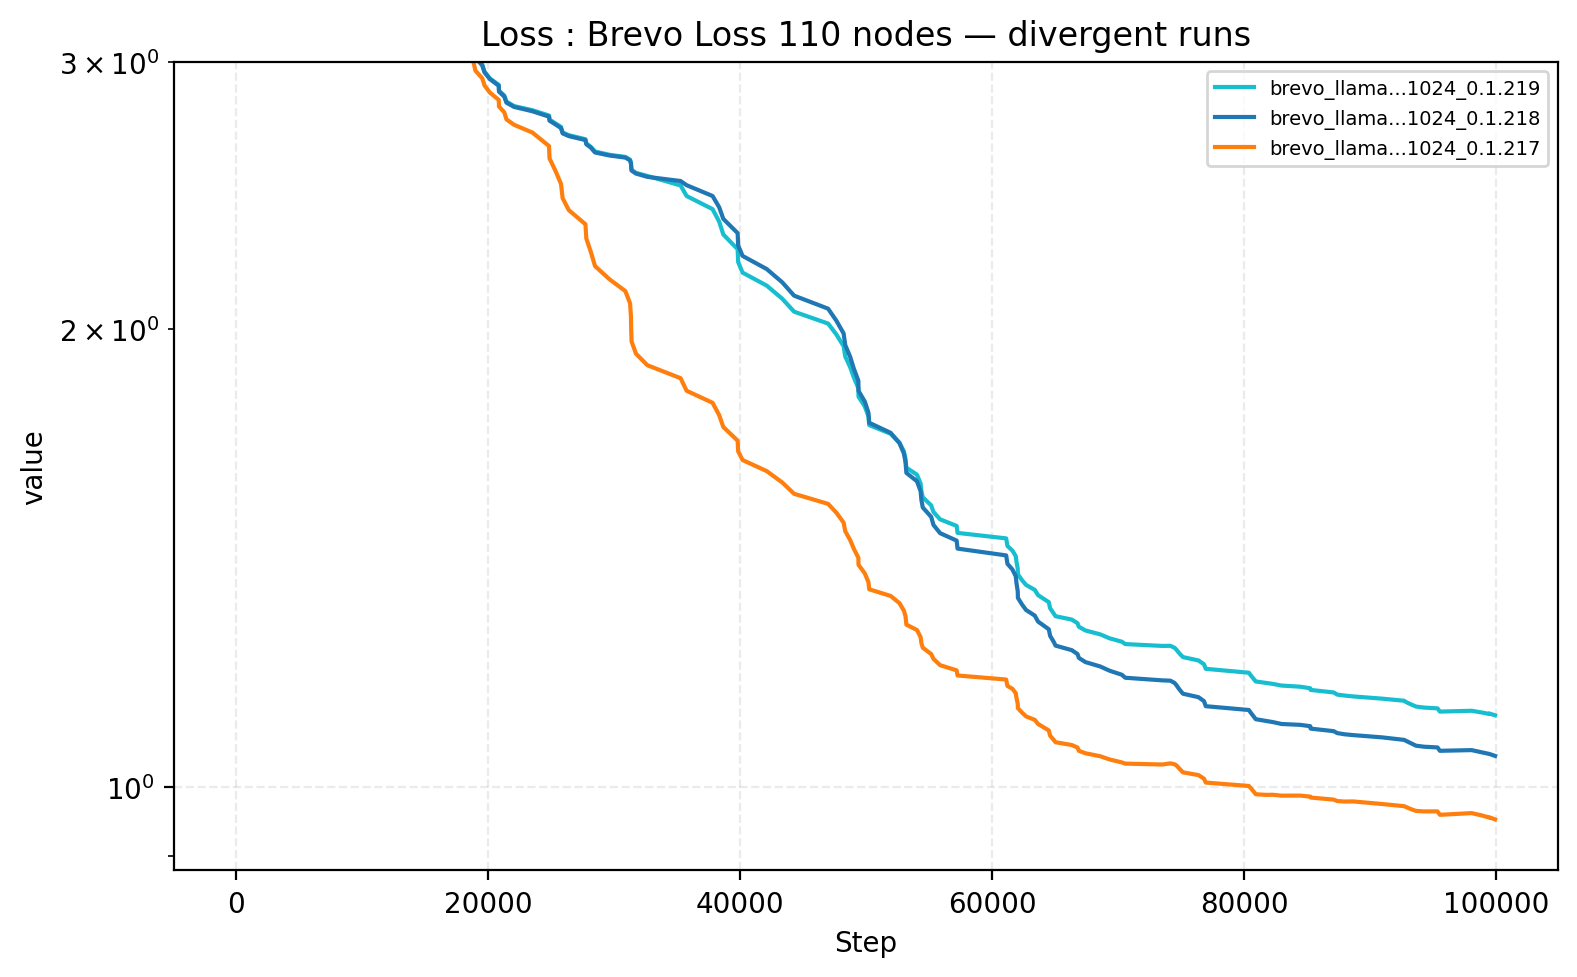
\includegraphics[width=0.7\linewidth]{march22_brevo_task_losses.png}
  \caption{Brevo training loss for three random seeds. Losses diverge across seeds,
    mirroring the instability observed on Depo.}
  \label{fig:brevo}
\end{figure}

\subsection{Discussion}
\label{sec:data:discussion}

Both Depo and Brevo can in principle identify a better-performing architecture when results
are averaged over many seeds. However, the high seed-to-seed variance makes individual
training runs unreliable proxies for studying \emph{training dynamics}. Metrics such as
gradient norms, representation scales, and activation kurtosis fluctuate as much
across seeds as they do across architectures, preventing meaningful comparison on a single
run. For dynamics analysis, a stable task such as standard text modeling is therefore
preferable.

% ---------------------------------------------------------------------------
\section{Canon Layers}
\label{sec:canon}
% ---------------------------------------------------------------------------

\subsection{Background}
\label{sec:canon:background}

A canon layer is a learned linear convolution applied to the last $k$ hidden-state vectors
along the sequence dimension. Let $\mathbf{h}_{t}$ be the hidden state at position $t$ and
$k$ be the kernel size. The canon output at position $t$ is
\[
  \tilde{\mathbf{h}}_t = \sum_{i=0}^{k-1} w_i \, \mathbf{h}_{t-i},
\]
where $\{w_i\}$ are scalar learned weights shared across the feature dimension.
Canon layers can be inserted at four positions within each transformer block:

\begin{itemize}
  \item \textbf{A} — before the self-attention sublayer (pre-attention),
  \item \textbf{B} — after the self-attention sublayer (post-attention),
  \item \textbf{C} — before the feed-forward sublayer (pre-FFN),
  \item \textbf{D} — after the feed-forward sublayer (post-FFN).
\end{itemize}

The key hyperparameters are the kernel size $k$, the weight initialization scheme, and
the subset of positions and layers in which canon is applied. Unless stated otherwise,
experiments use Canon-ABCD (all four positions) across all transformer layers.

\subsection{Performance vs.\ Llama Baseline}
\label{sec:canon:perf}

\begin{figure}[h]
  \centering
  \begin{subfigure}[b]{0.48\linewidth}
    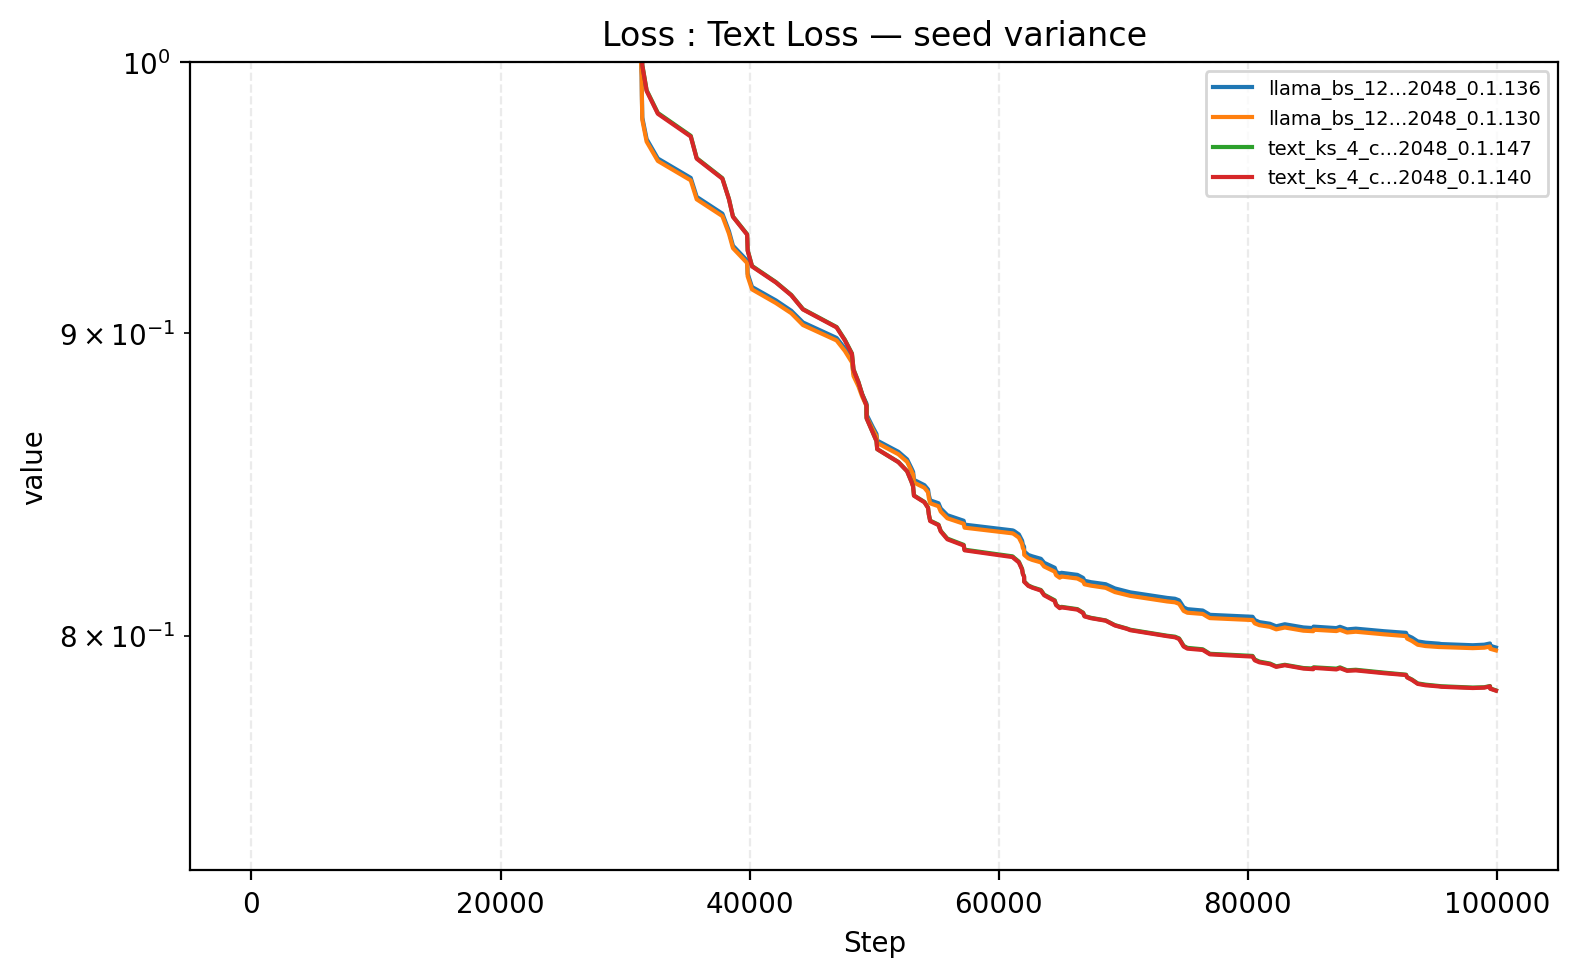
\includegraphics[width=\linewidth]{march09_stability_text_loss.png}
    \caption{Canon vs.\ Llama on text modeling.}
    \label{fig:canon_vs_llama}
  \end{subfigure}
  \hfill
  \begin{subfigure}[b]{0.48\linewidth}
    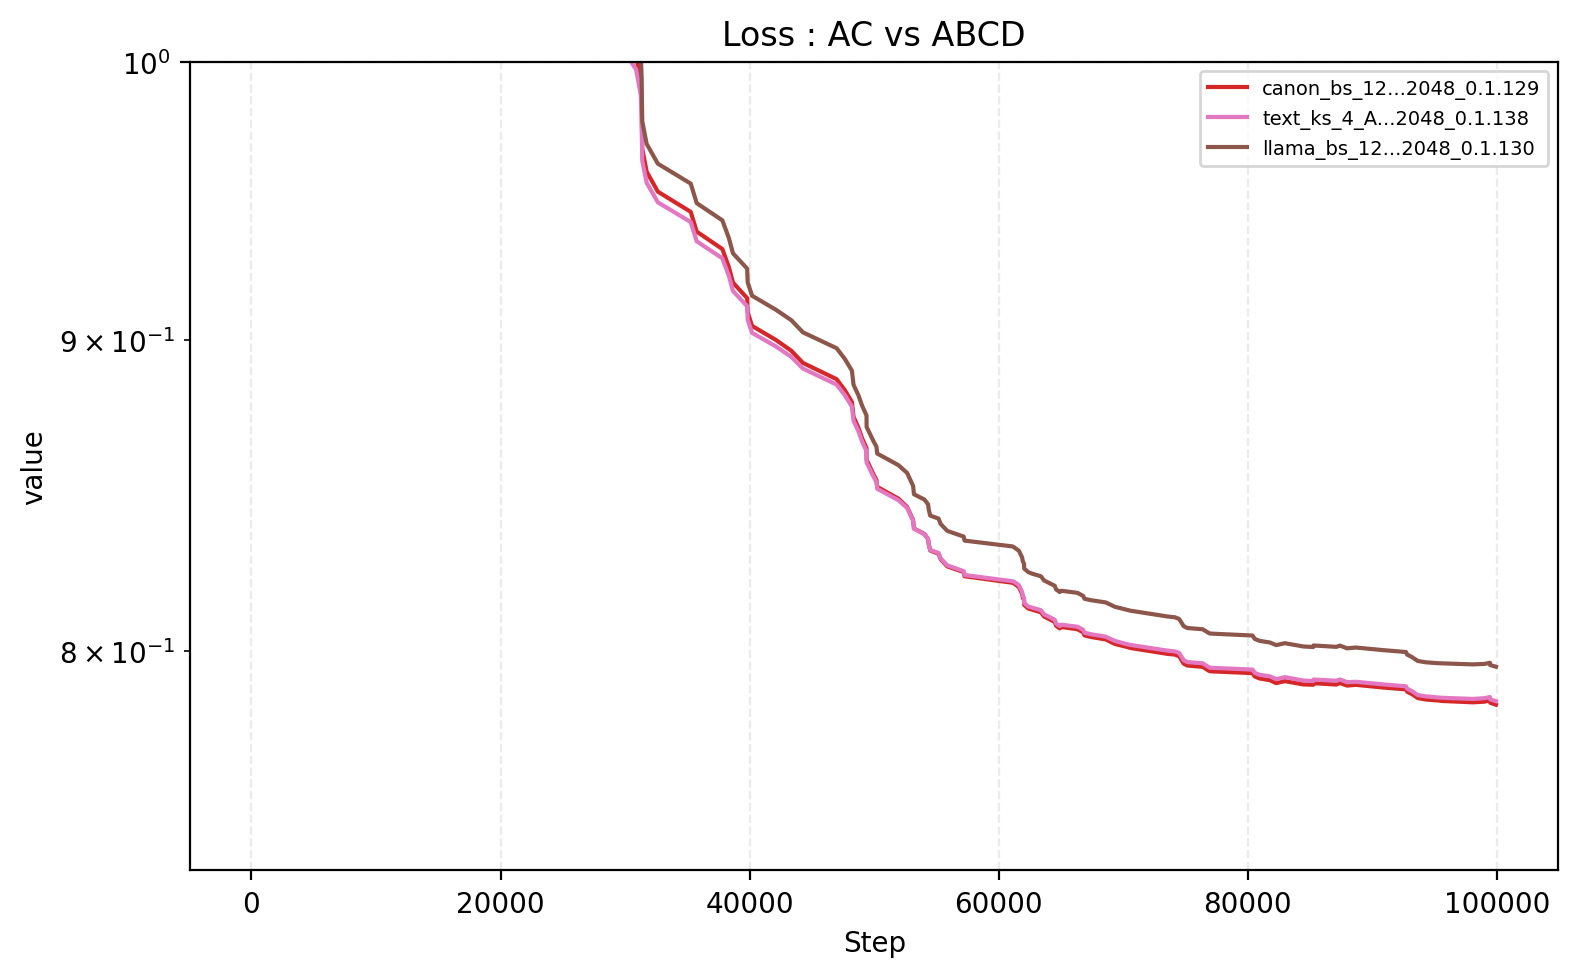
\includegraphics[width=\linewidth]{march09_dynamics_loss_ac_vs_abcd.png}
    \caption{Canon-AC vs.\ Canon-ABCD vs.\ Baseline.}
    \label{fig:ac_vs_abcd}
  \end{subfigure}
  \caption{Left: Canon overtakes the Llama baseline around step 50\,000 and reaches a
    final loss of 0.776 vs.\ 0.790. Right: Using only the pre-attention and pre-FFN
    canon positions (AC) captures nearly all of the gain over the baseline.}
  \label{fig:canon_perf}
\end{figure}

On the FineWeb-Edu text modeling task, Canon is slower to start than Llama but overtakes
the baseline around step 50\,000 and achieves a final loss of \textbf{0.776} compared to
\textbf{0.790} for the Llama baseline (Figure~\ref{fig:canon_vs_llama}).

A position ablation (Figure~\ref{fig:ac_vs_abcd}) shows that Canon-AC (positions A and C
only) performs nearly as well as the full Canon-ABCD configuration. Adding post-attention
(B) and post-FFN (D) canons provides only marginal additional benefit.

\subsection{Ablations}
\label{sec:canon:ablations}

\subsubsection{Kernel Size}

\begin{figure}[h]
  \centering
  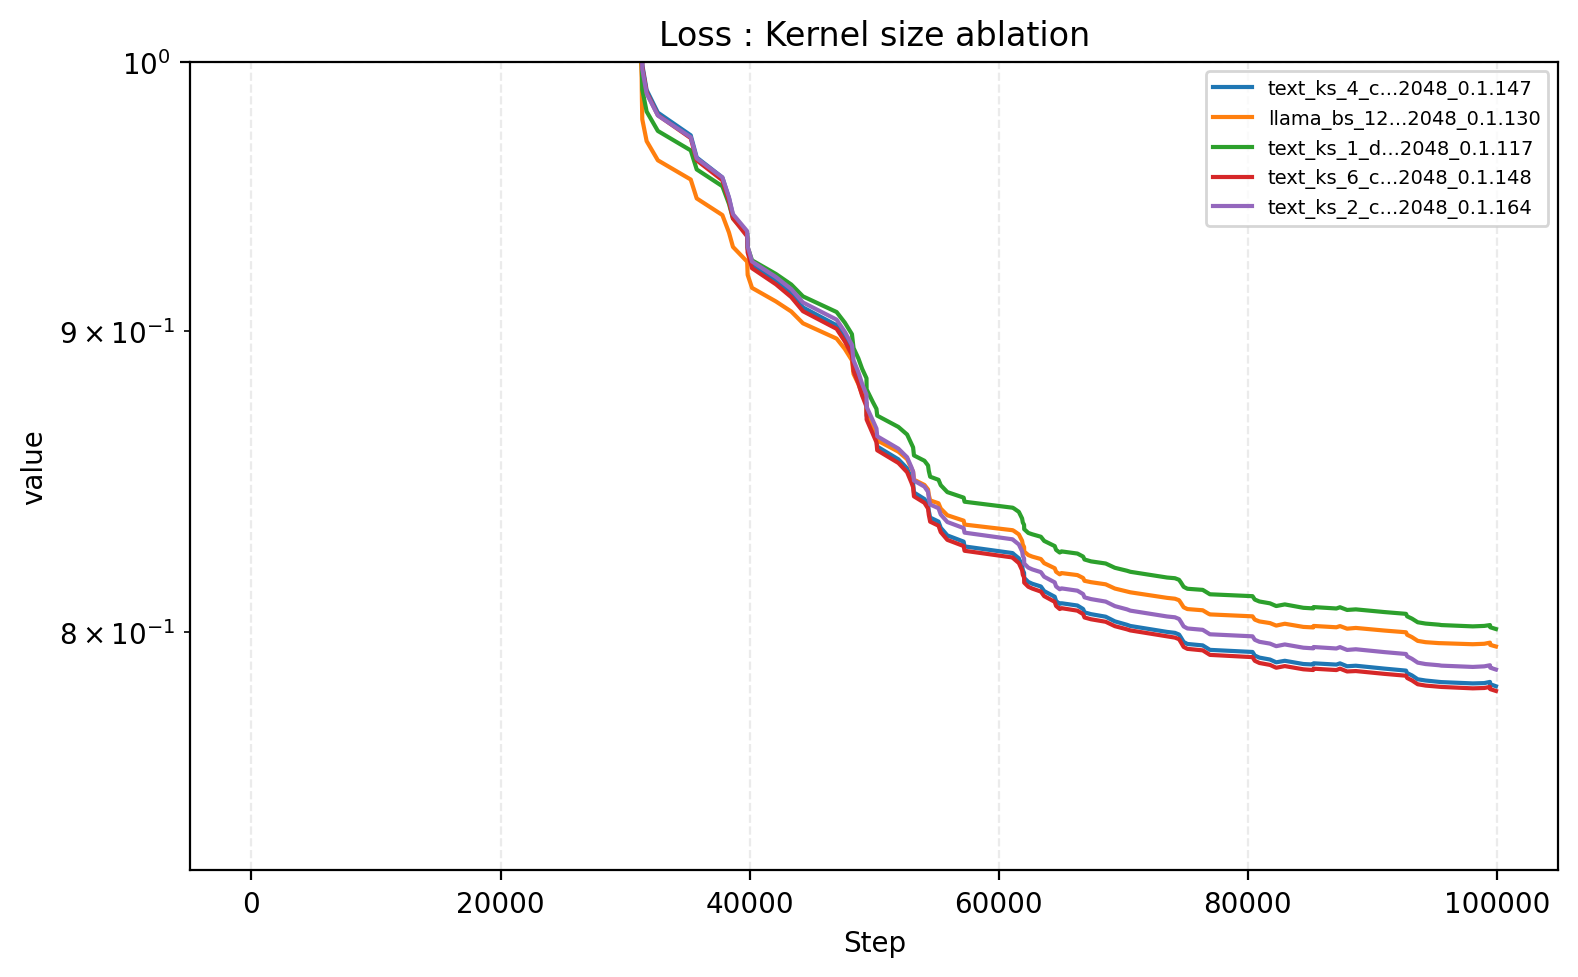
\includegraphics[width=0.7\linewidth]{march09_kernel_size_ablation_loss.png}
  \caption{Training loss on text modeling for kernel sizes 1, 2, 4, 6, and the Llama
    baseline. Larger kernels consistently outperform smaller ones; $k{=}1$ is even
    worse than no canon.}
  \label{fig:ks_ablation}
\end{figure}

Figure~\ref{fig:ks_ablation} compares kernel sizes $k \in \{1, 2, 4, 6\}$ against the
Llama baseline. A kernel of size 1 reduces to a pointwise rescaling and performs
worse than no canon at all, confirming that cross-token mixing is essential. Performance
improves monotonically with kernel size up to $k{=}6$.

\subsubsection{Weight Initialization}

\begin{figure}[h]
  \centering
  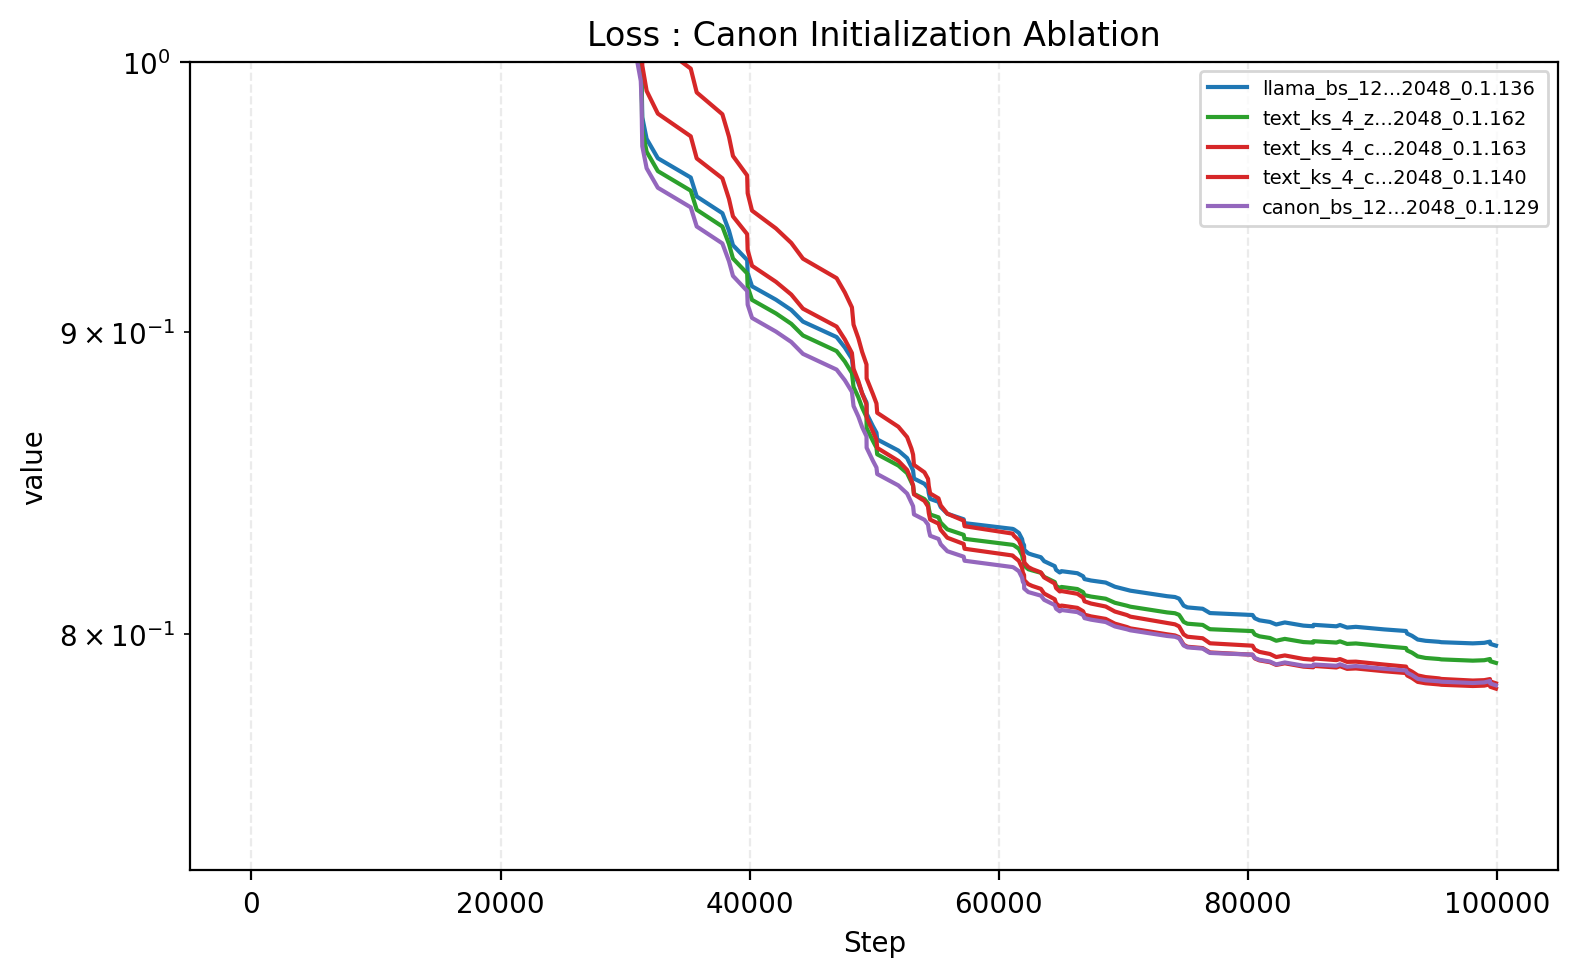
\includegraphics[width=0.7\linewidth]{march09_initialization_ablation_loss.png}
  \caption{Initialization ablation on text modeling. All canon variants outperform the
    Llama baseline; $1/k$ constant initialization is best.}
  \label{fig:init_ablation}
\end{figure}

We compare four initialization schemes for the canon weights $\{w_i\}$
(Figure~\ref{fig:init_ablation}):

\begin{itemize}
  \item \texttt{const\_var\_sqrt}: constant $1/k$,
  \item \texttt{const\_var}: constant $1/\sqrt{k}$,
  \item \texttt{default\_init}: $\mathcal{U}[-\fract{1}{\sqrt{k}}, \fract{1}{\sqrt{k}}]$,
  \item \texttt{zeros\_init}: all zeros.
\end{itemize}

Notably, even zero initialization beats the Llama baseline, indicating
that the architectural benefit of canon is not entirely dependent on initialization.
The $1/k$ scheme (equal weight per shift, normalized by kernel size) is the strongest.

\subsubsection{Canon Position Within the Network}

\begin{figure}[h]
  \centering
  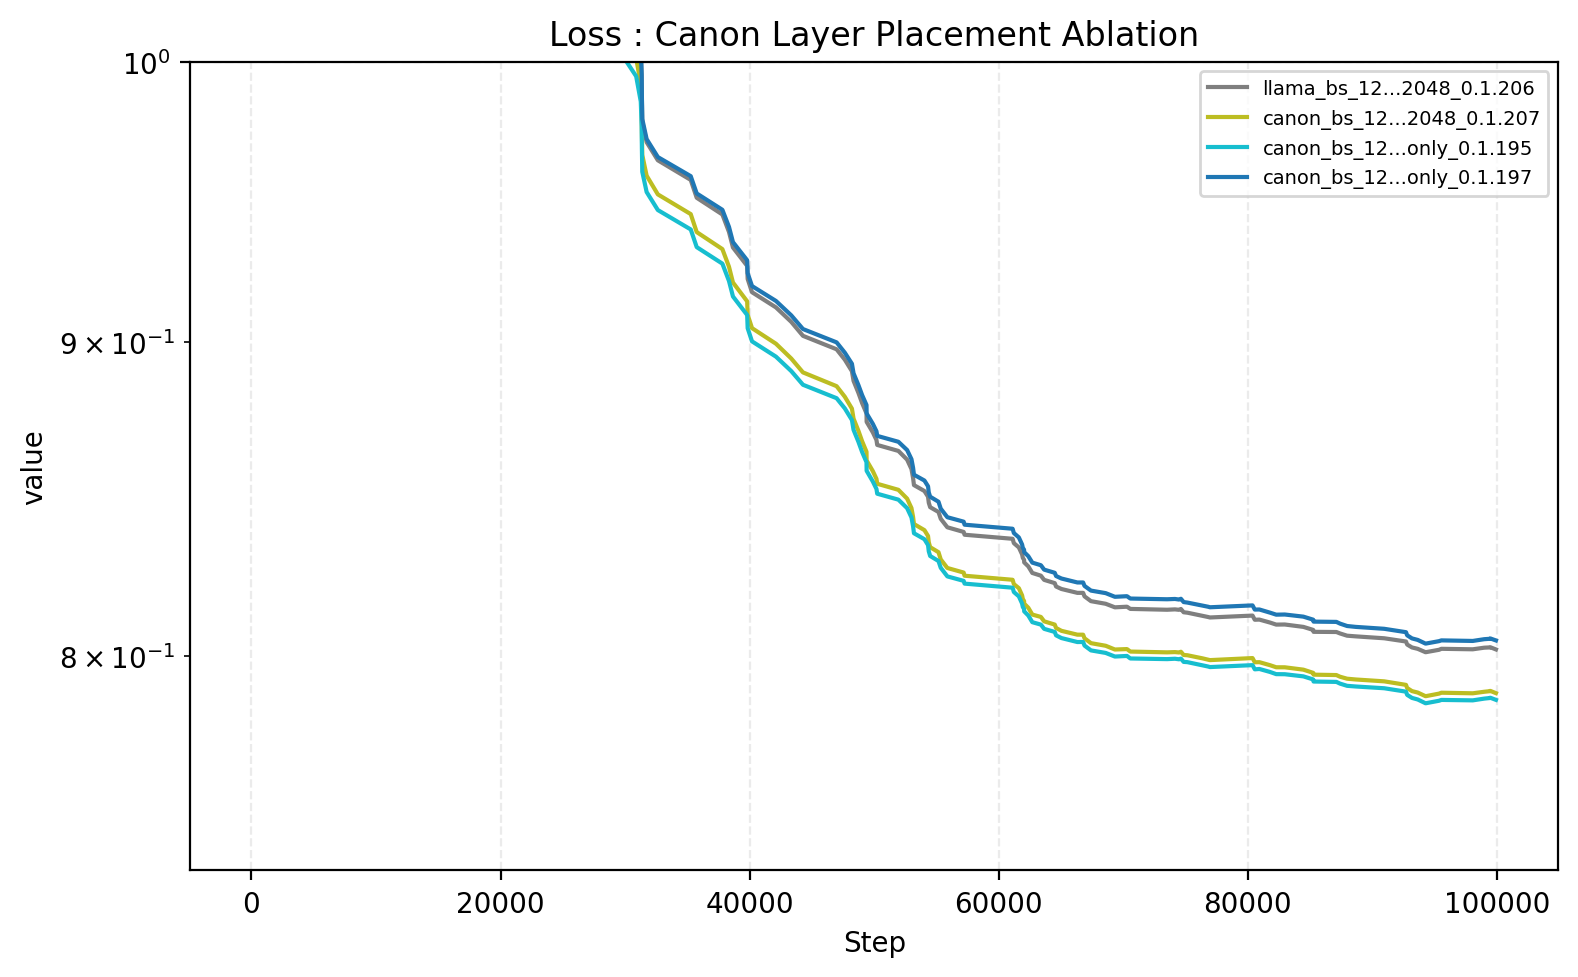
\includegraphics[width=0.7\linewidth]{ablation_canon_layer_loss.png}
  \caption{Loss for canon applied to all layers, the first layer only, the last layer
    only, and the Llama baseline.}
  \label{fig:layer_ablation}
\end{figure}

Figure~\ref{fig:layer_ablation} compares inserting canon across all transformer layers
versus restricting it to the first or last layer only. Placing canon in all layers
provides the strongest benefit; single-layer variants still improve over the baseline
but to a lesser degree.

\subsubsection{Normalization Type}

\begin{figure}[h]
  \centering
  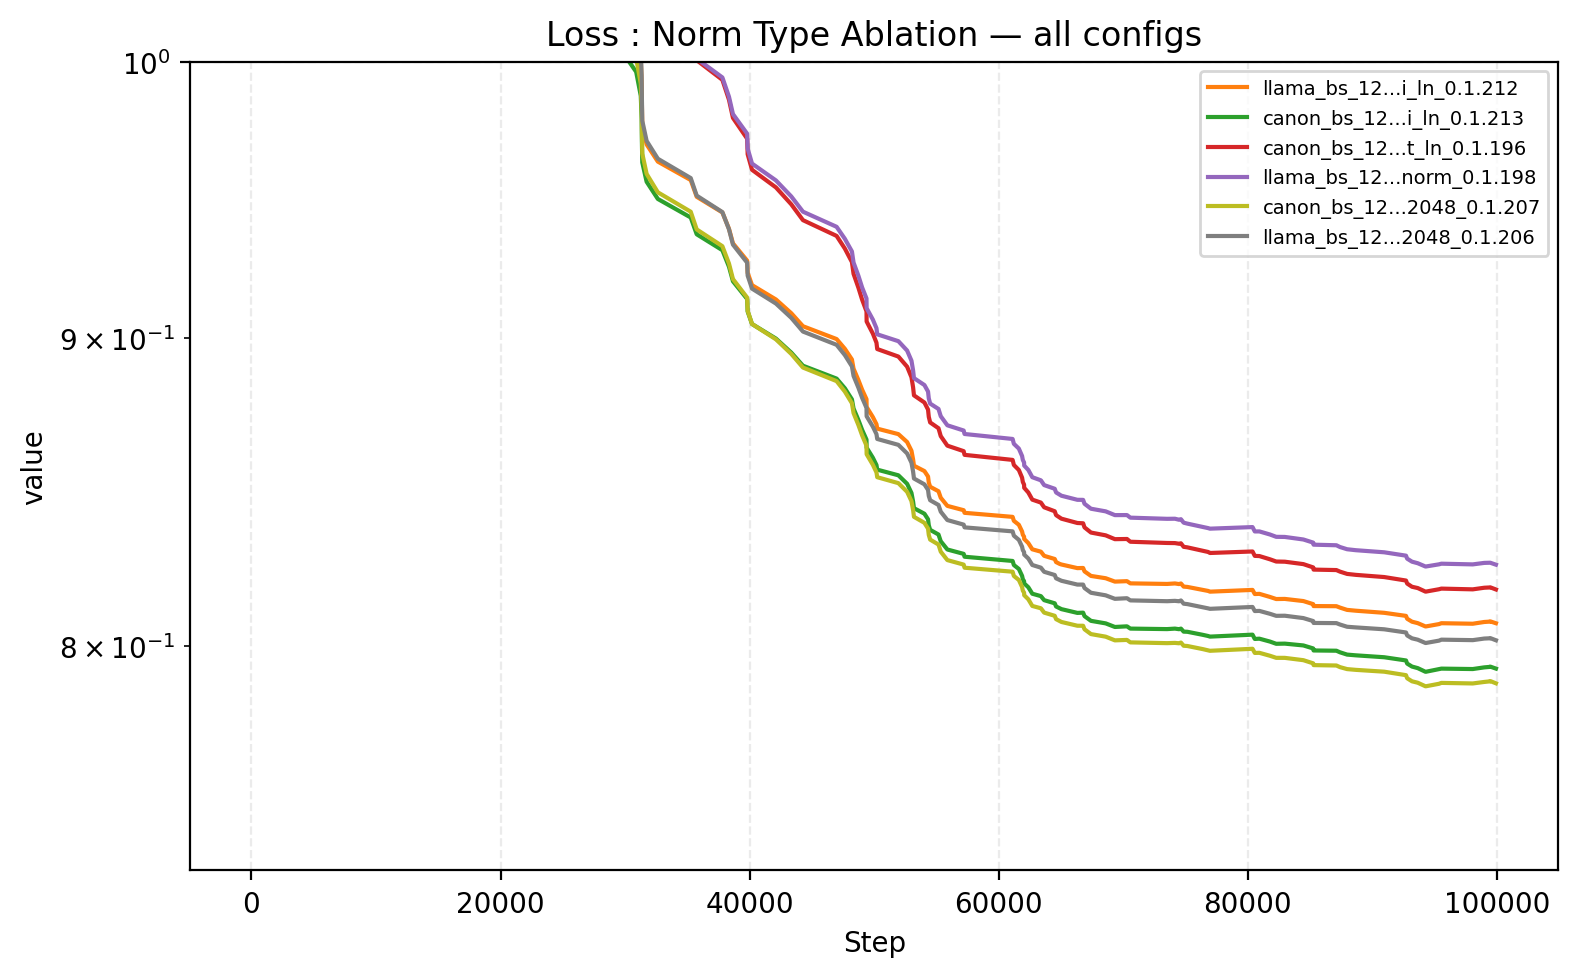
\includegraphics[width=\linewidth]{norm_types_loss.png}
  \caption{Training loss for Canon and Llama under Pre-LN, Post-LN, and Peri-LN
    normalization. Canon consistently outperforms the same-normalization Llama baseline
    across all three schemes.}
  \label{fig:norm_types}
\end{figure}

Canon's benefit is not specific to a single normalization scheme.
Figure~\ref{fig:norm_types} shows that Canon outperforms the corresponding Llama baseline
under Pre-LN, Post-LN, and Peri-LN normalization. Figures~\ref{fig:norm_gradients}
and~\ref{fig:norm_repr_scale} show the associated gradient and representation-scale
dynamics per normalization type.

\begin{figure}[h]
  \centering
  \begin{subfigure}[b]{0.32\linewidth}
    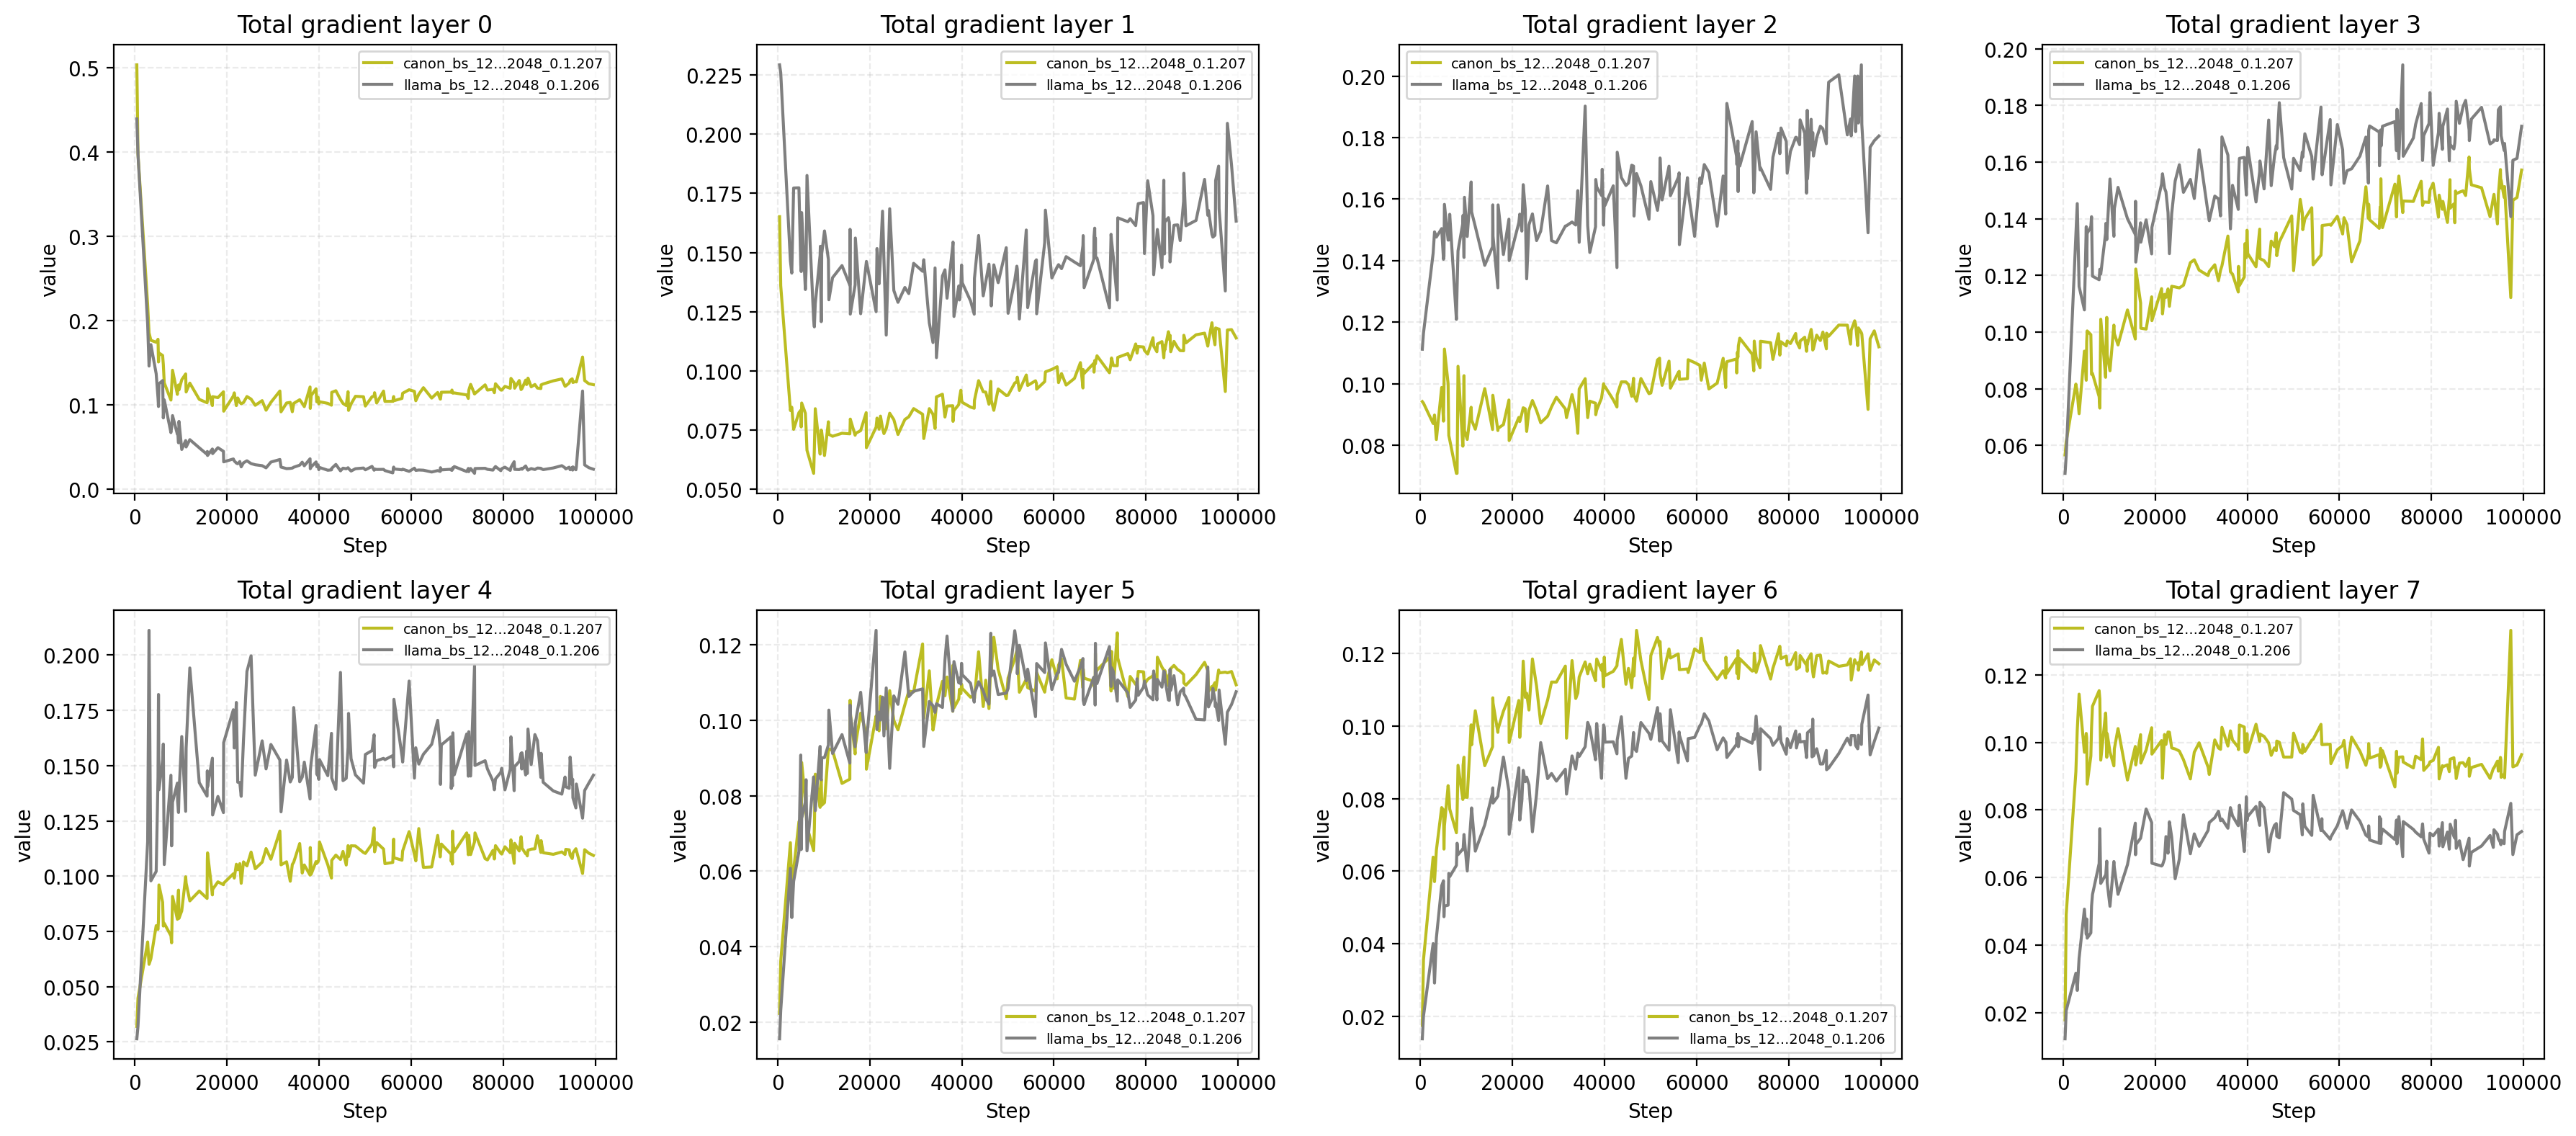
\includegraphics[width=\linewidth]{norm_gradients_pre_ln.png}
    \caption{Pre-LN gradients.}
  \end{subfigure}
  \hfill
  \begin{subfigure}[b]{0.32\linewidth}
    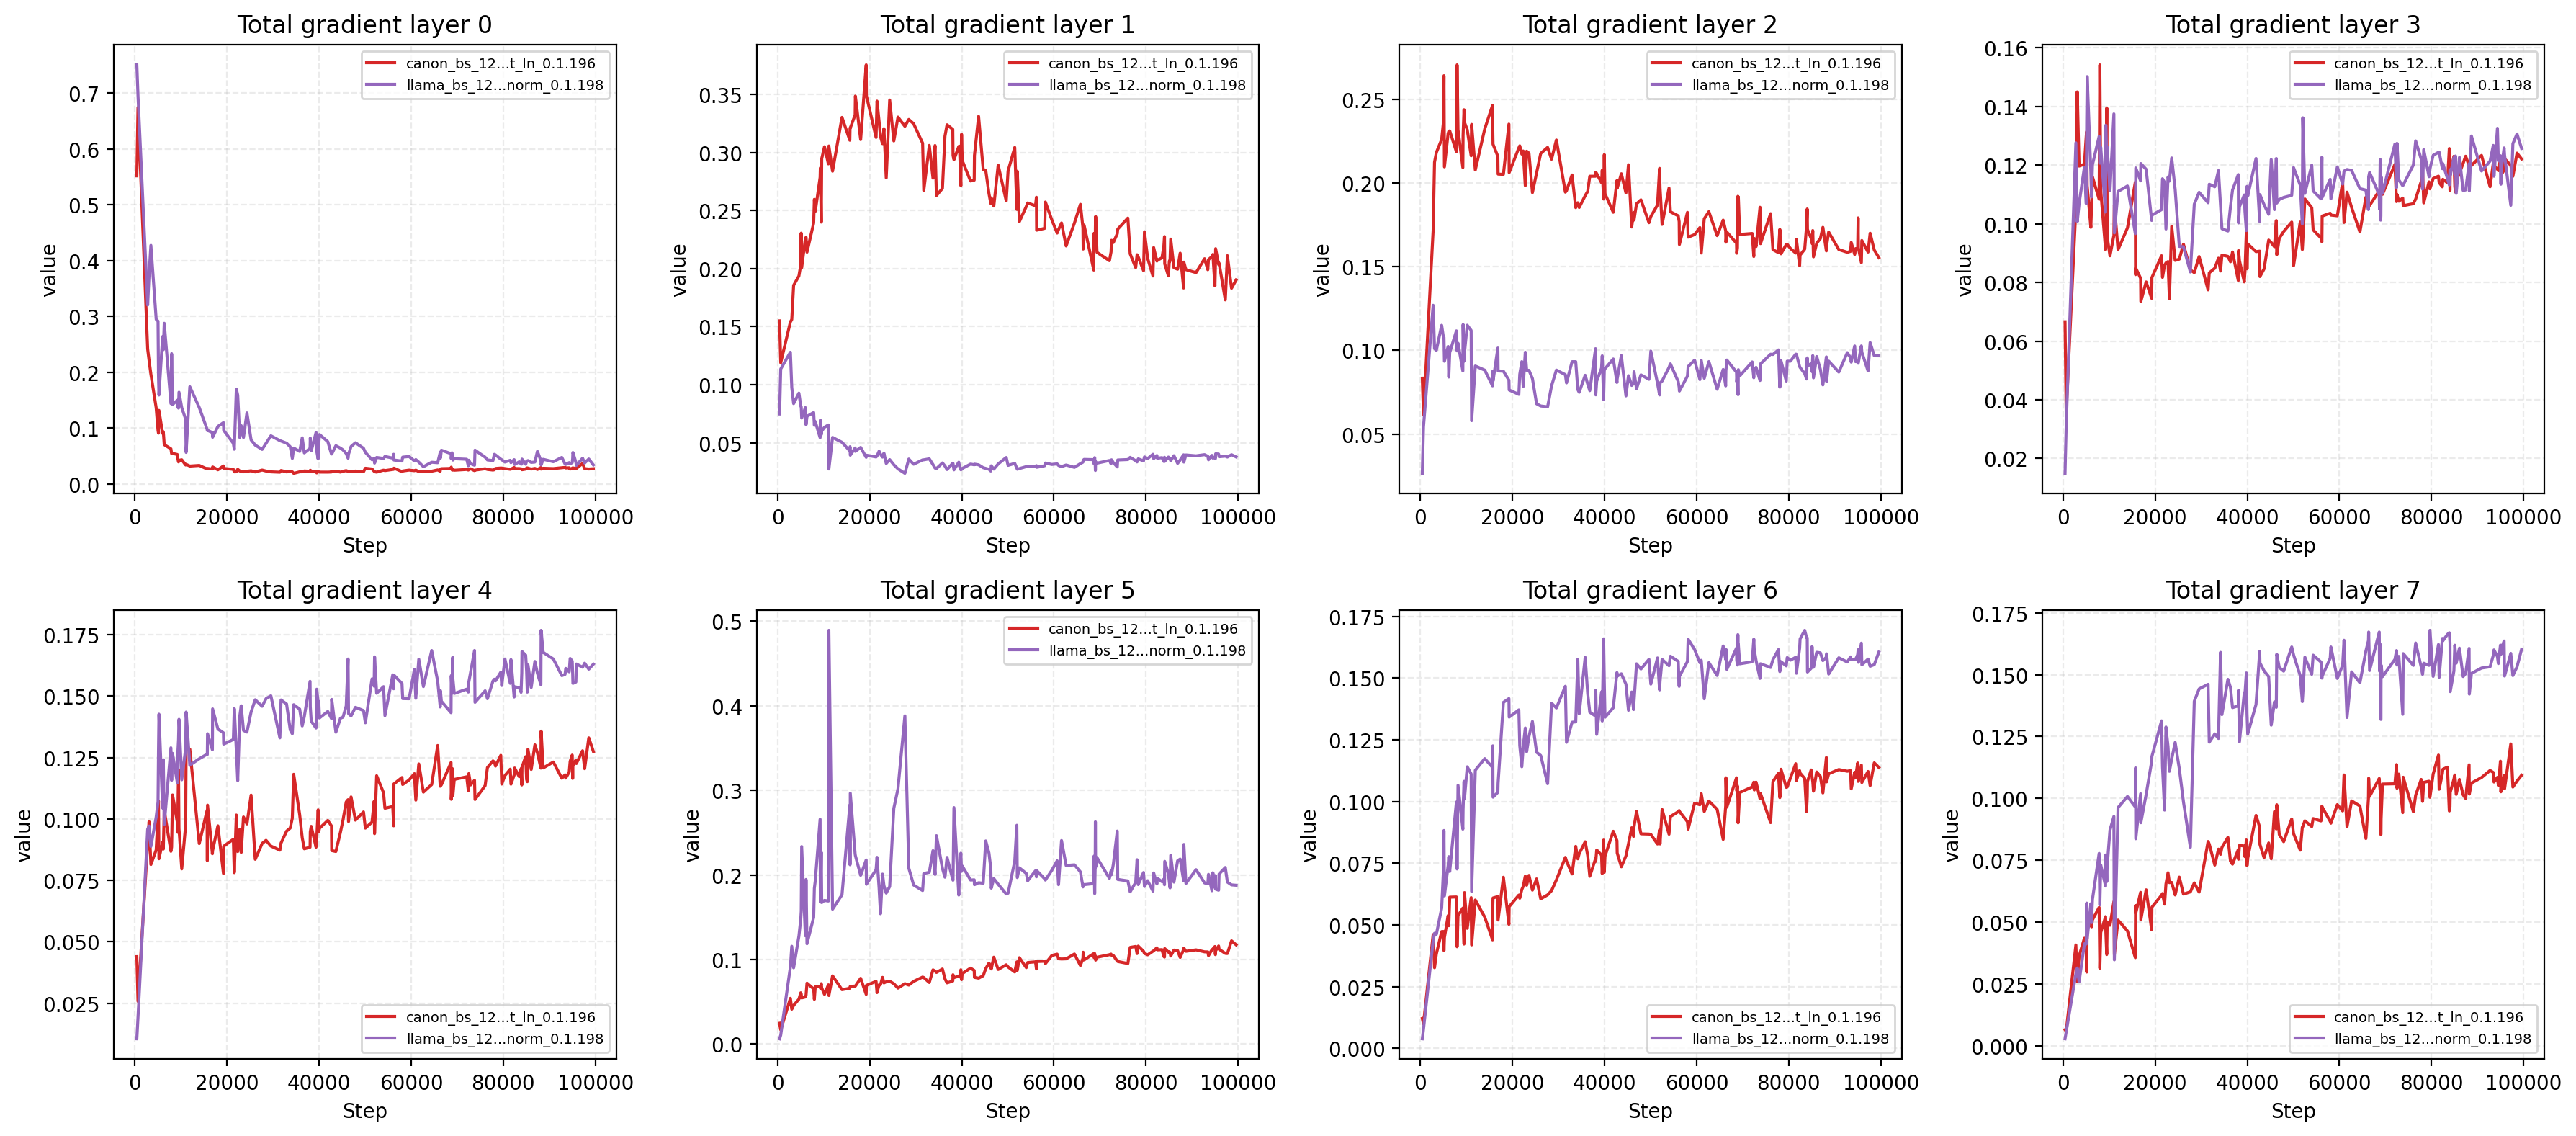
\includegraphics[width=\linewidth]{norm_gradients_post_ln.png}
    \caption{Post-LN gradients.}
  \end{subfigure}
  \hfill
  \begin{subfigure}[b]{0.32\linewidth}
    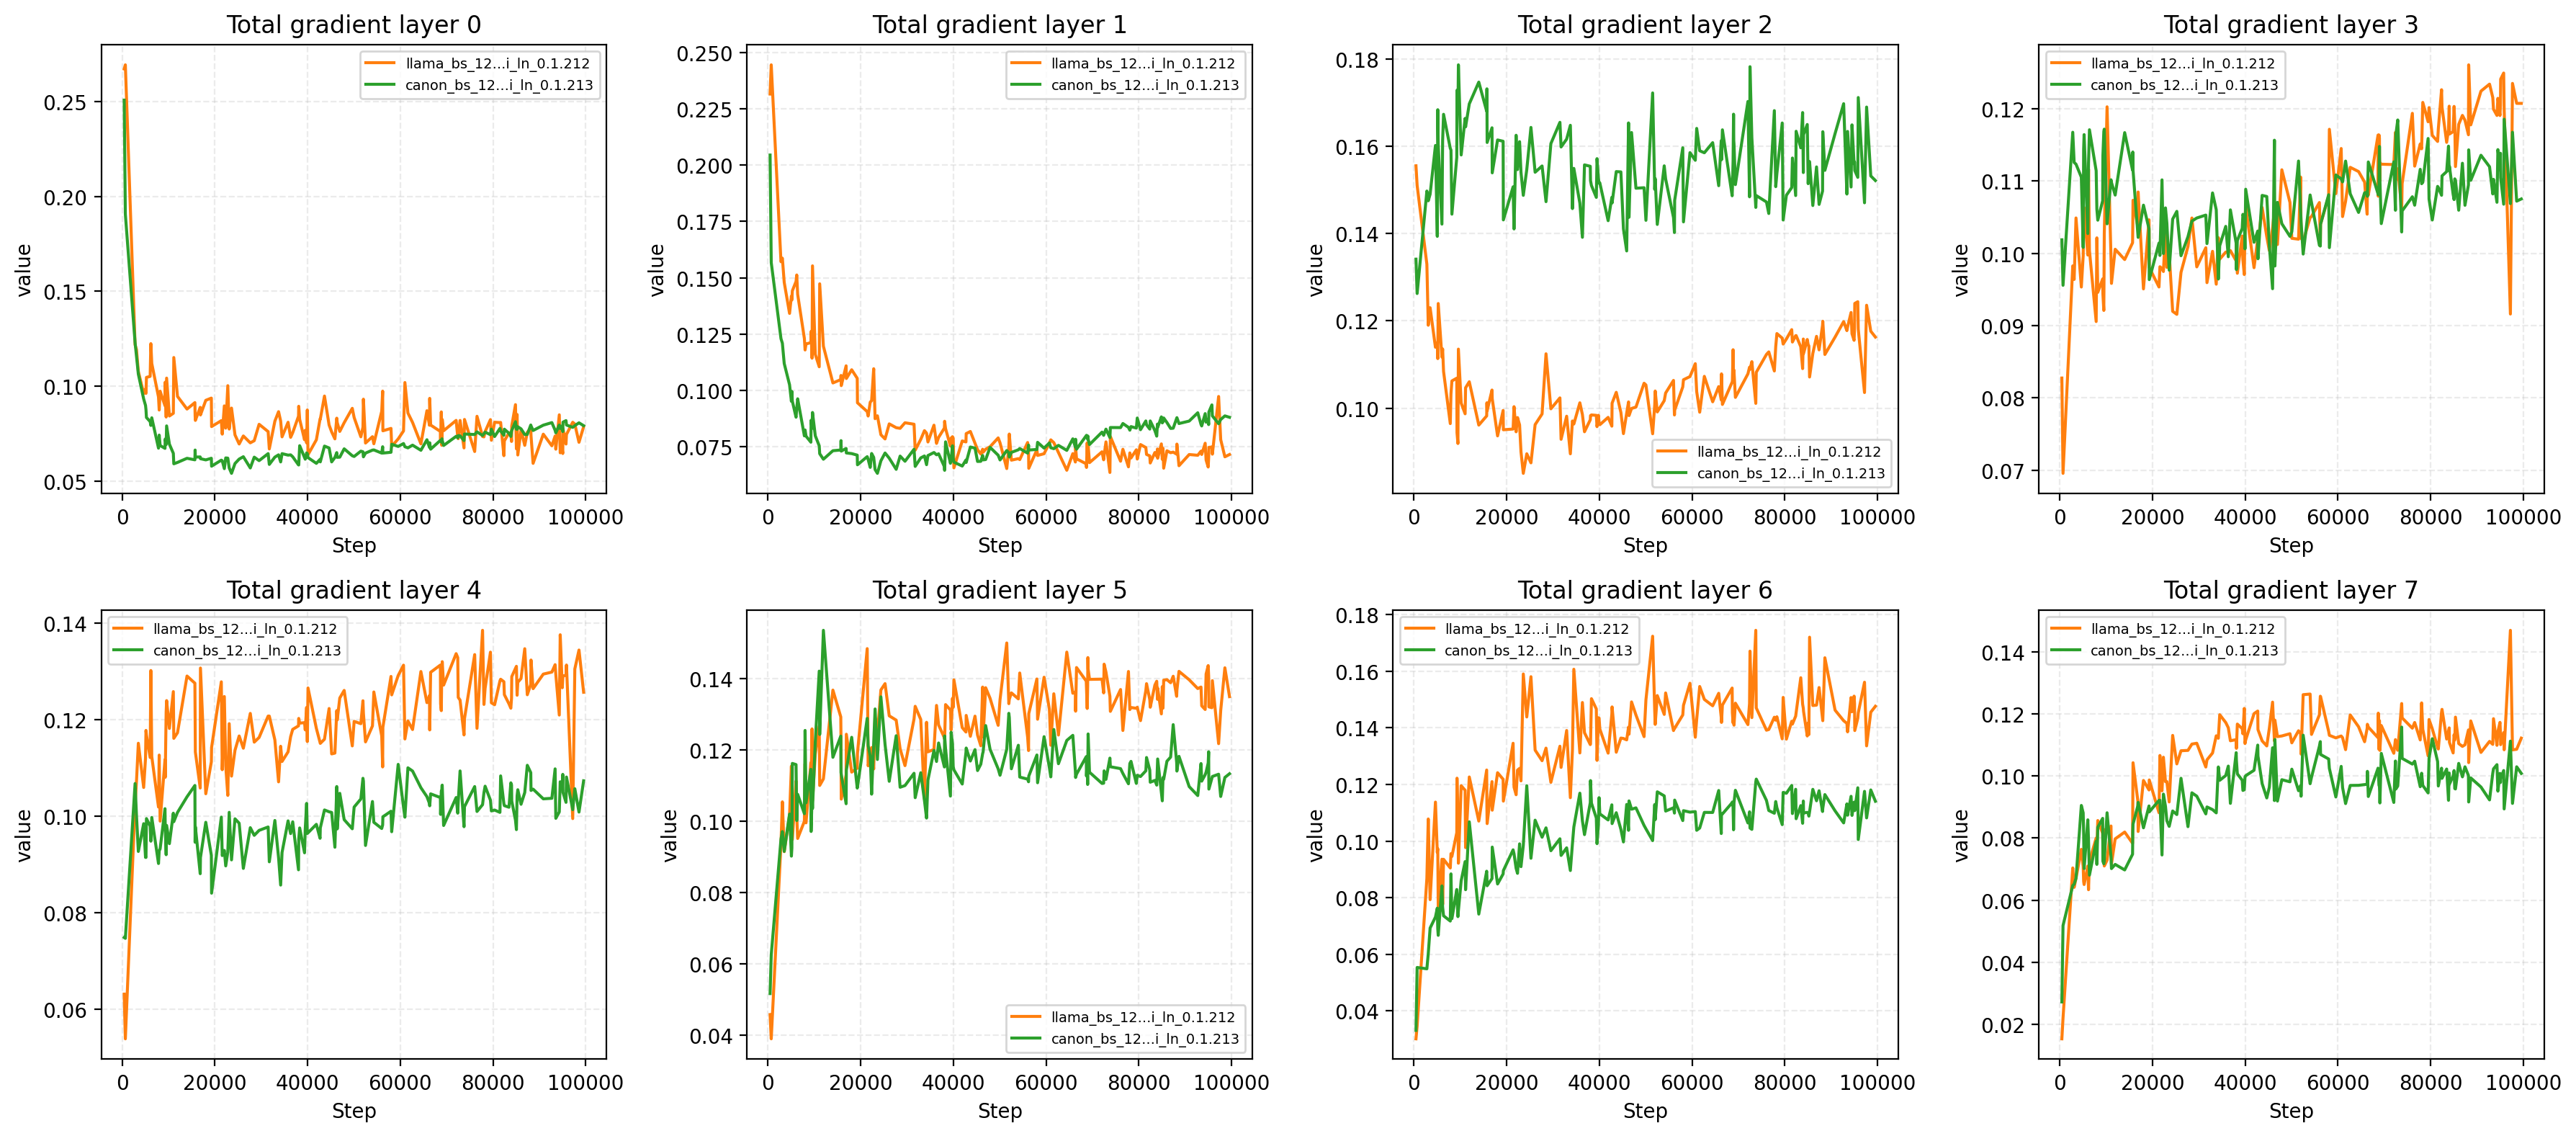
\includegraphics[width=\linewidth]{norm_gradients_peri_ln.png}
    \caption{Peri-LN gradients.}
  \end{subfigure}
  \caption{Per-layer gradient contributions for Canon and Llama under each normalization
    type.}
  \label{fig:norm_gradients}
\end{figure}

\begin{figure}[h]
  \centering
  \begin{subfigure}[b]{0.32\linewidth}
    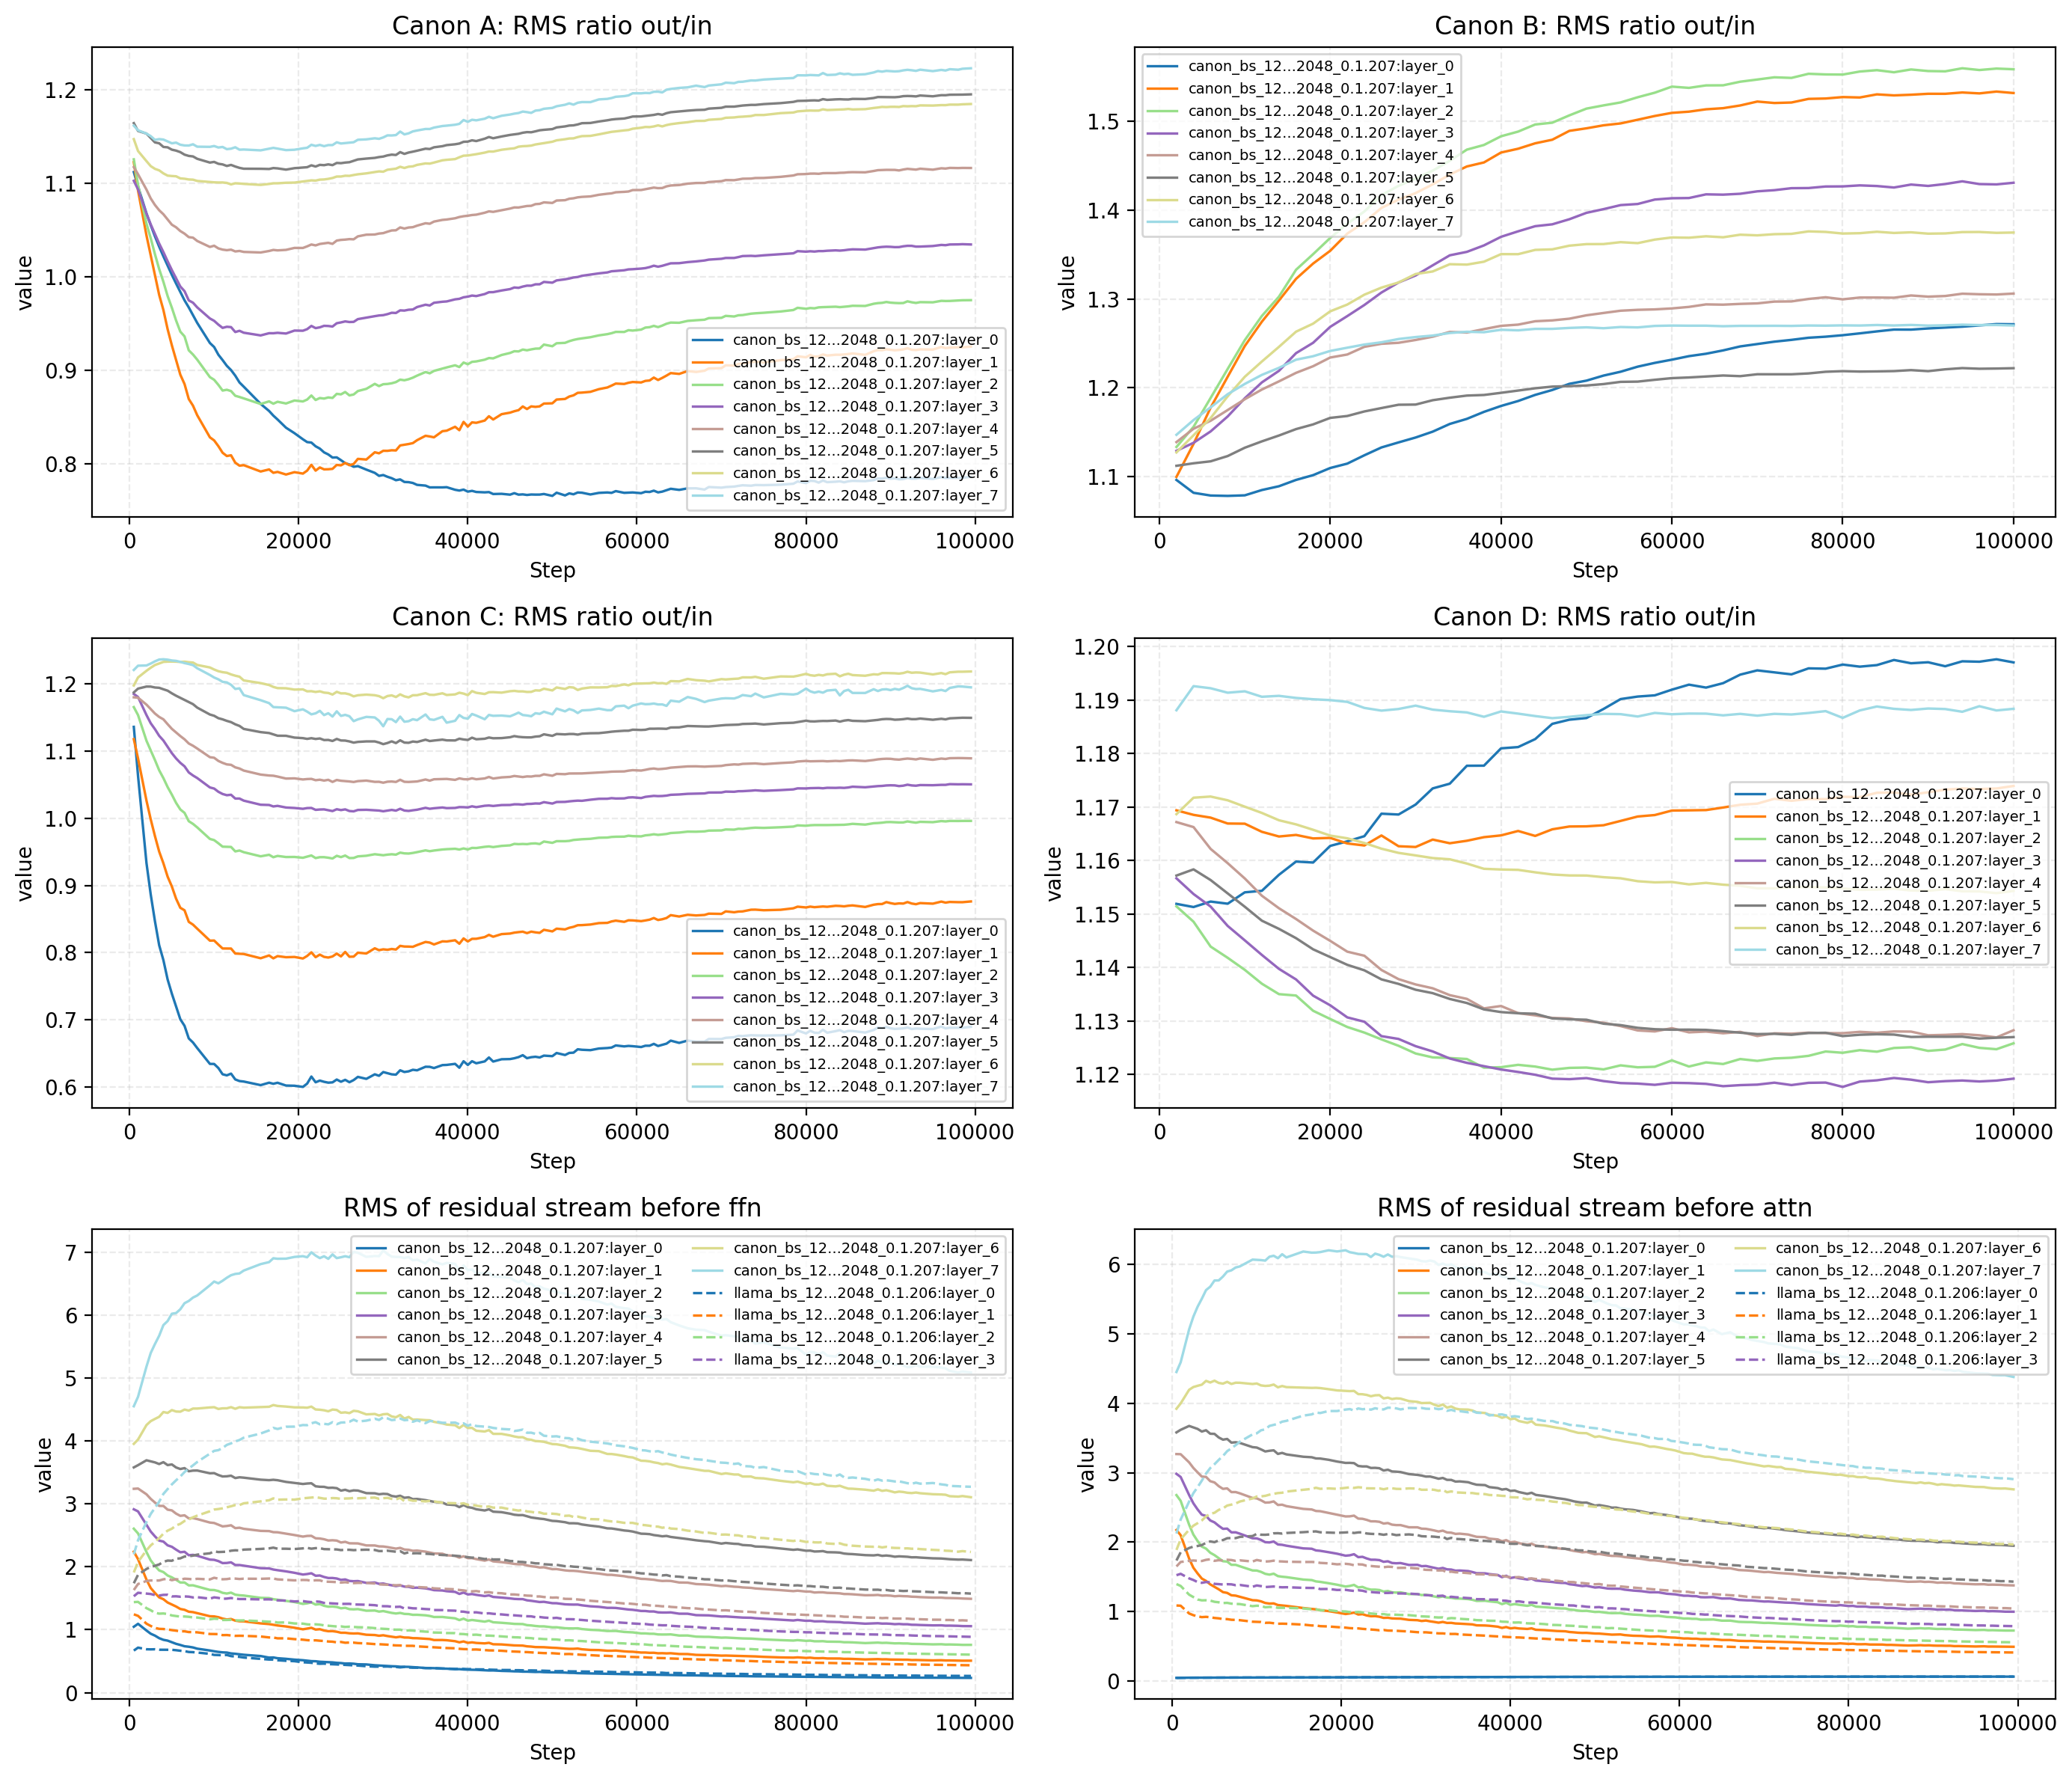
\includegraphics[width=\linewidth]{norm_repr_scale_pre_ln.png}
    \caption{Pre-LN repr.\ scale.}
  \end{subfigure}
  \hfill
  \begin{subfigure}[b]{0.32\linewidth}
    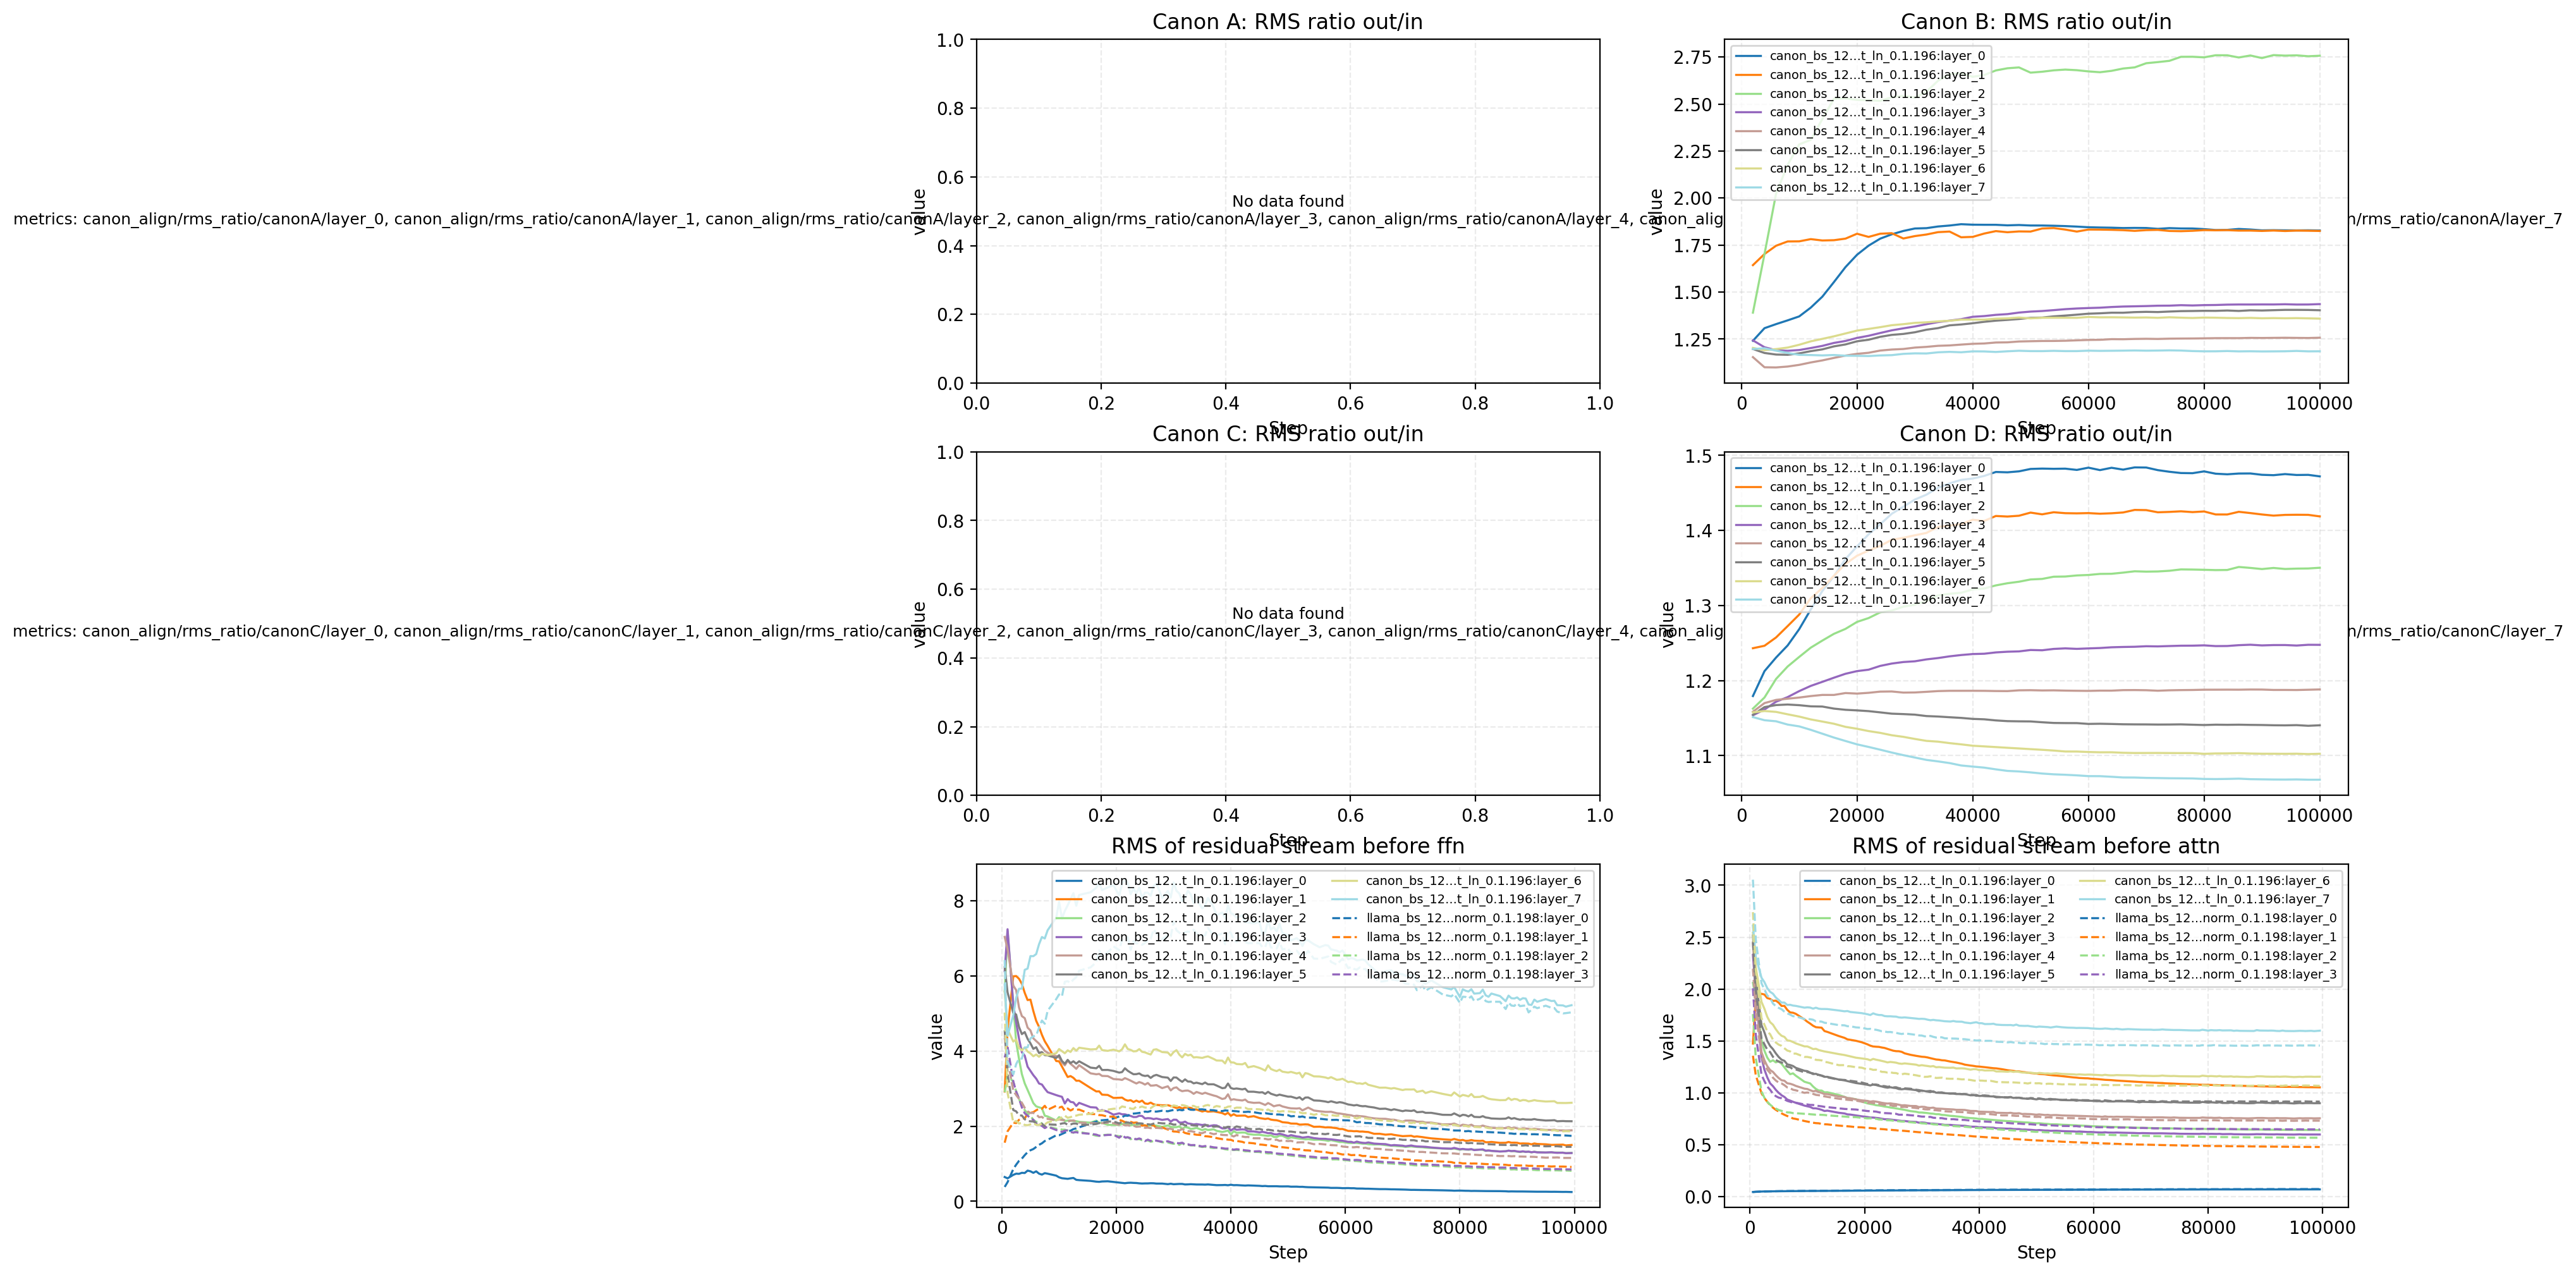
\includegraphics[width=\linewidth]{norm_repr_scale_post_ln.png}
    \caption{Post-LN repr.\ scale.}
  \end{subfigure}
  \hfill
  \begin{subfigure}[b]{0.32\linewidth}
    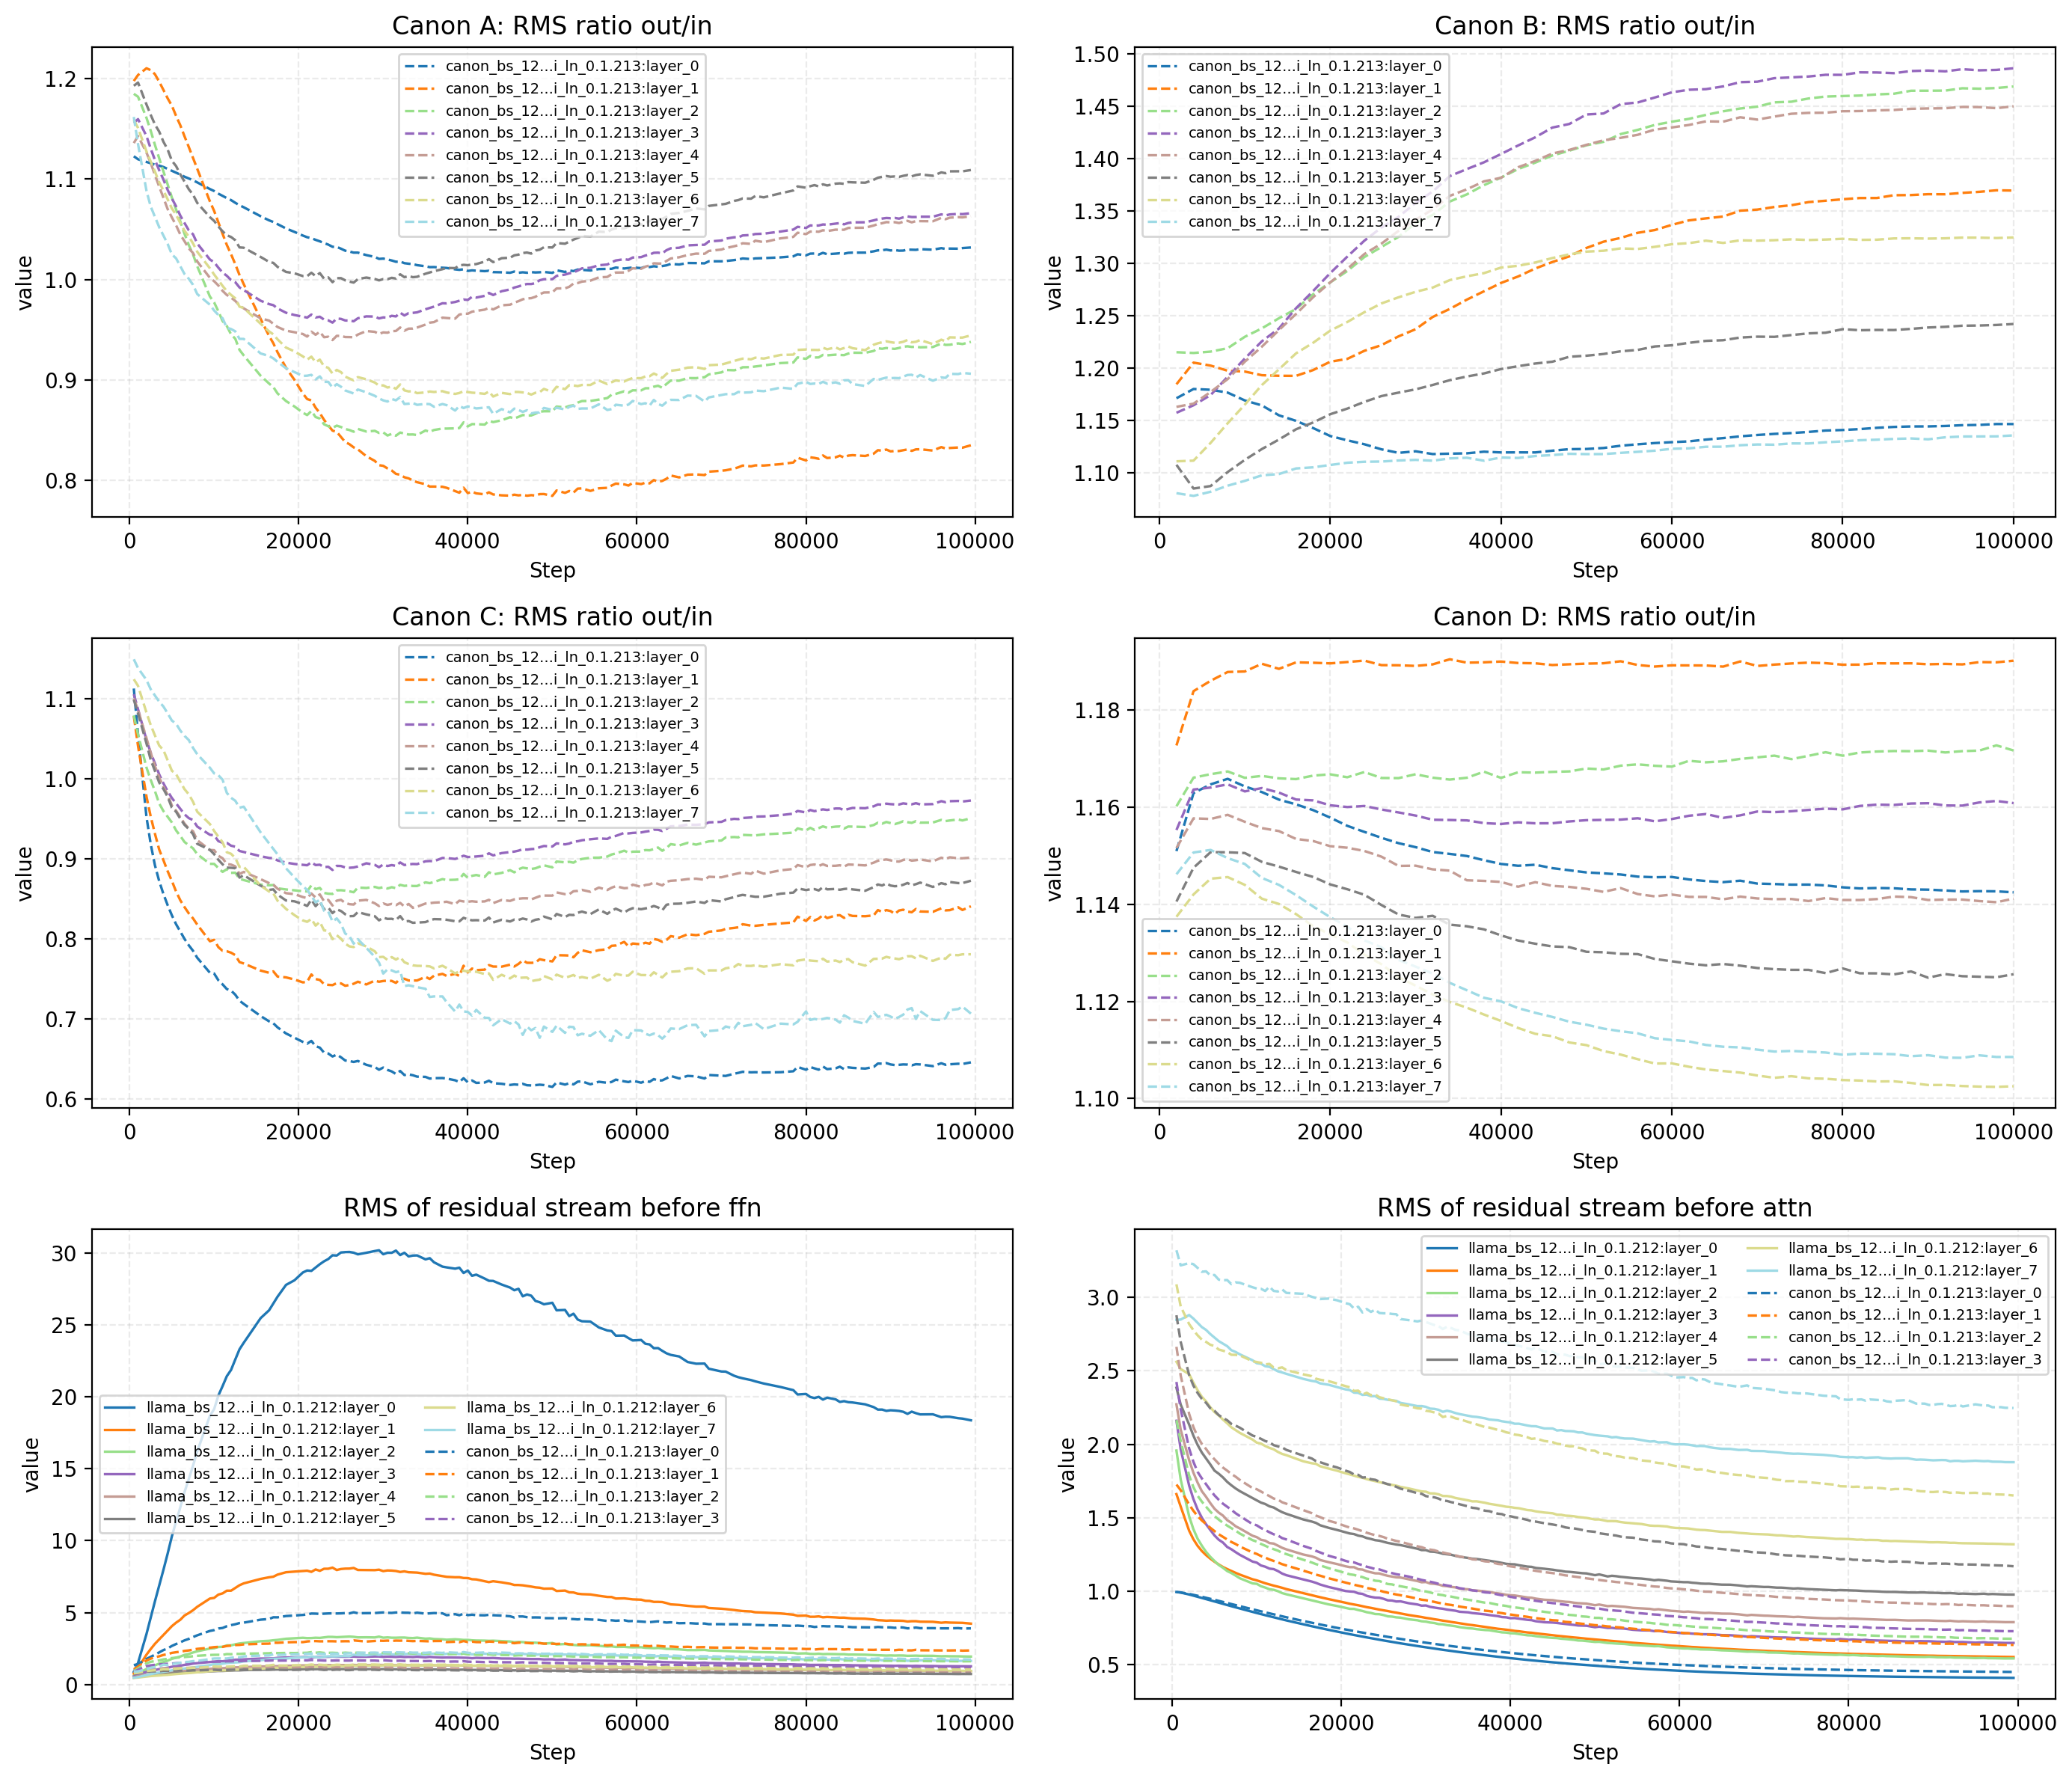
\includegraphics[width=\linewidth]{norm_repr_scale_peri_ln.png}
    \caption{Peri-LN repr.\ scale.}
  \end{subfigure}
  \caption{Residual stream RMS scale per layer for Canon and Llama under each
    normalization type.}
  \label{fig:norm_repr_scale}
\end{figure}

\subsection{Training Dynamics}
\label{sec:canon:dynamics}

All dynamics figures below compare a Canon-ABCD model (\texttt{ks=4}, default
initialization) against the Llama baseline on the text modeling task.

\subsubsection{Canon Weights: Farther Shifts Receive Larger Weights}

\begin{figure}[h]
  \centering
  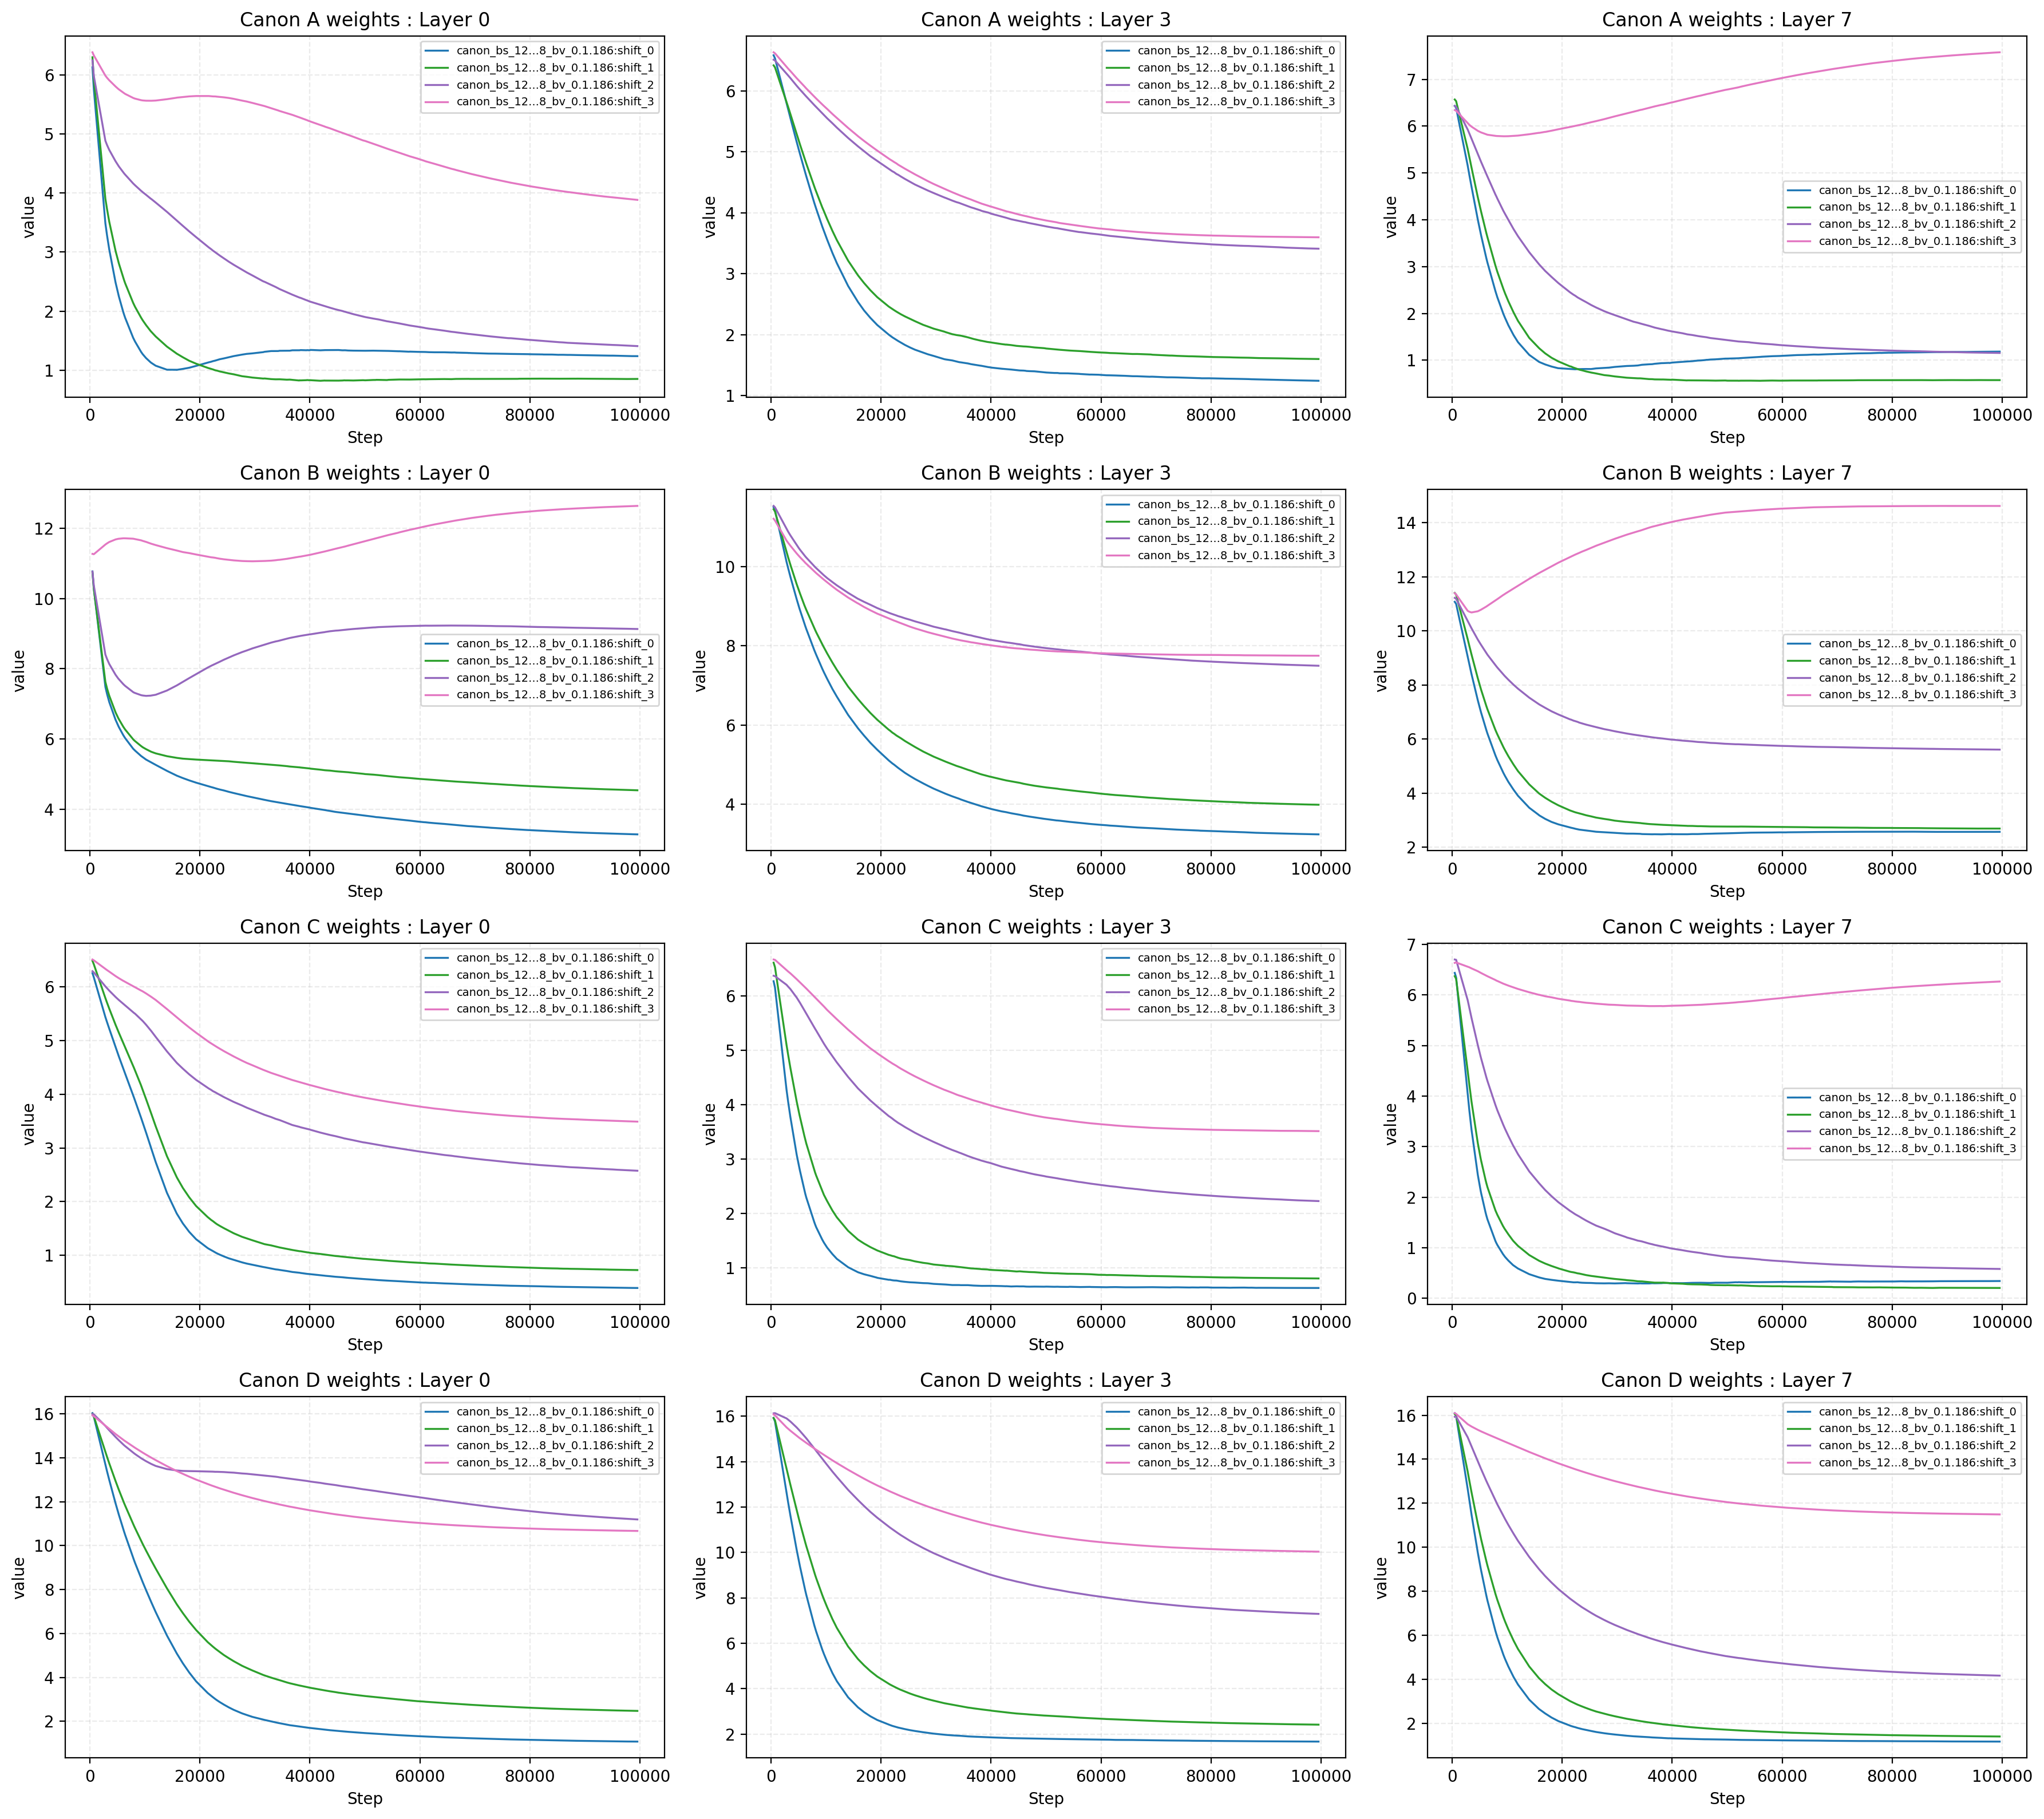
\includegraphics[width=\linewidth]{dynamics_canon_weights_layerwise.png}
  \caption{Learned canon weights for types A, B, C, D at layers 0, 3, and 7 throughout
    training. Weights for larger shifts (more distant tokens) are consistently larger than
    weights for shorter shifts.}
  \label{fig:canon_weights}
\end{figure}

Figure~\ref{fig:canon_weights} shows the learned scalar weights $\{w_i\}$ for each
canon type and a representative set of layers. Across all types and layers, weights
corresponding to larger shifts (e.g., $i{=}3$) are larger than those for smaller shifts
(e.g., $i{=}1$). This suggests the model actively learns to integrate context from
distant positions rather than relying on the immediately preceding token.

\subsubsection{Representation Scaling}

\begin{figure}[h]
  \centering
  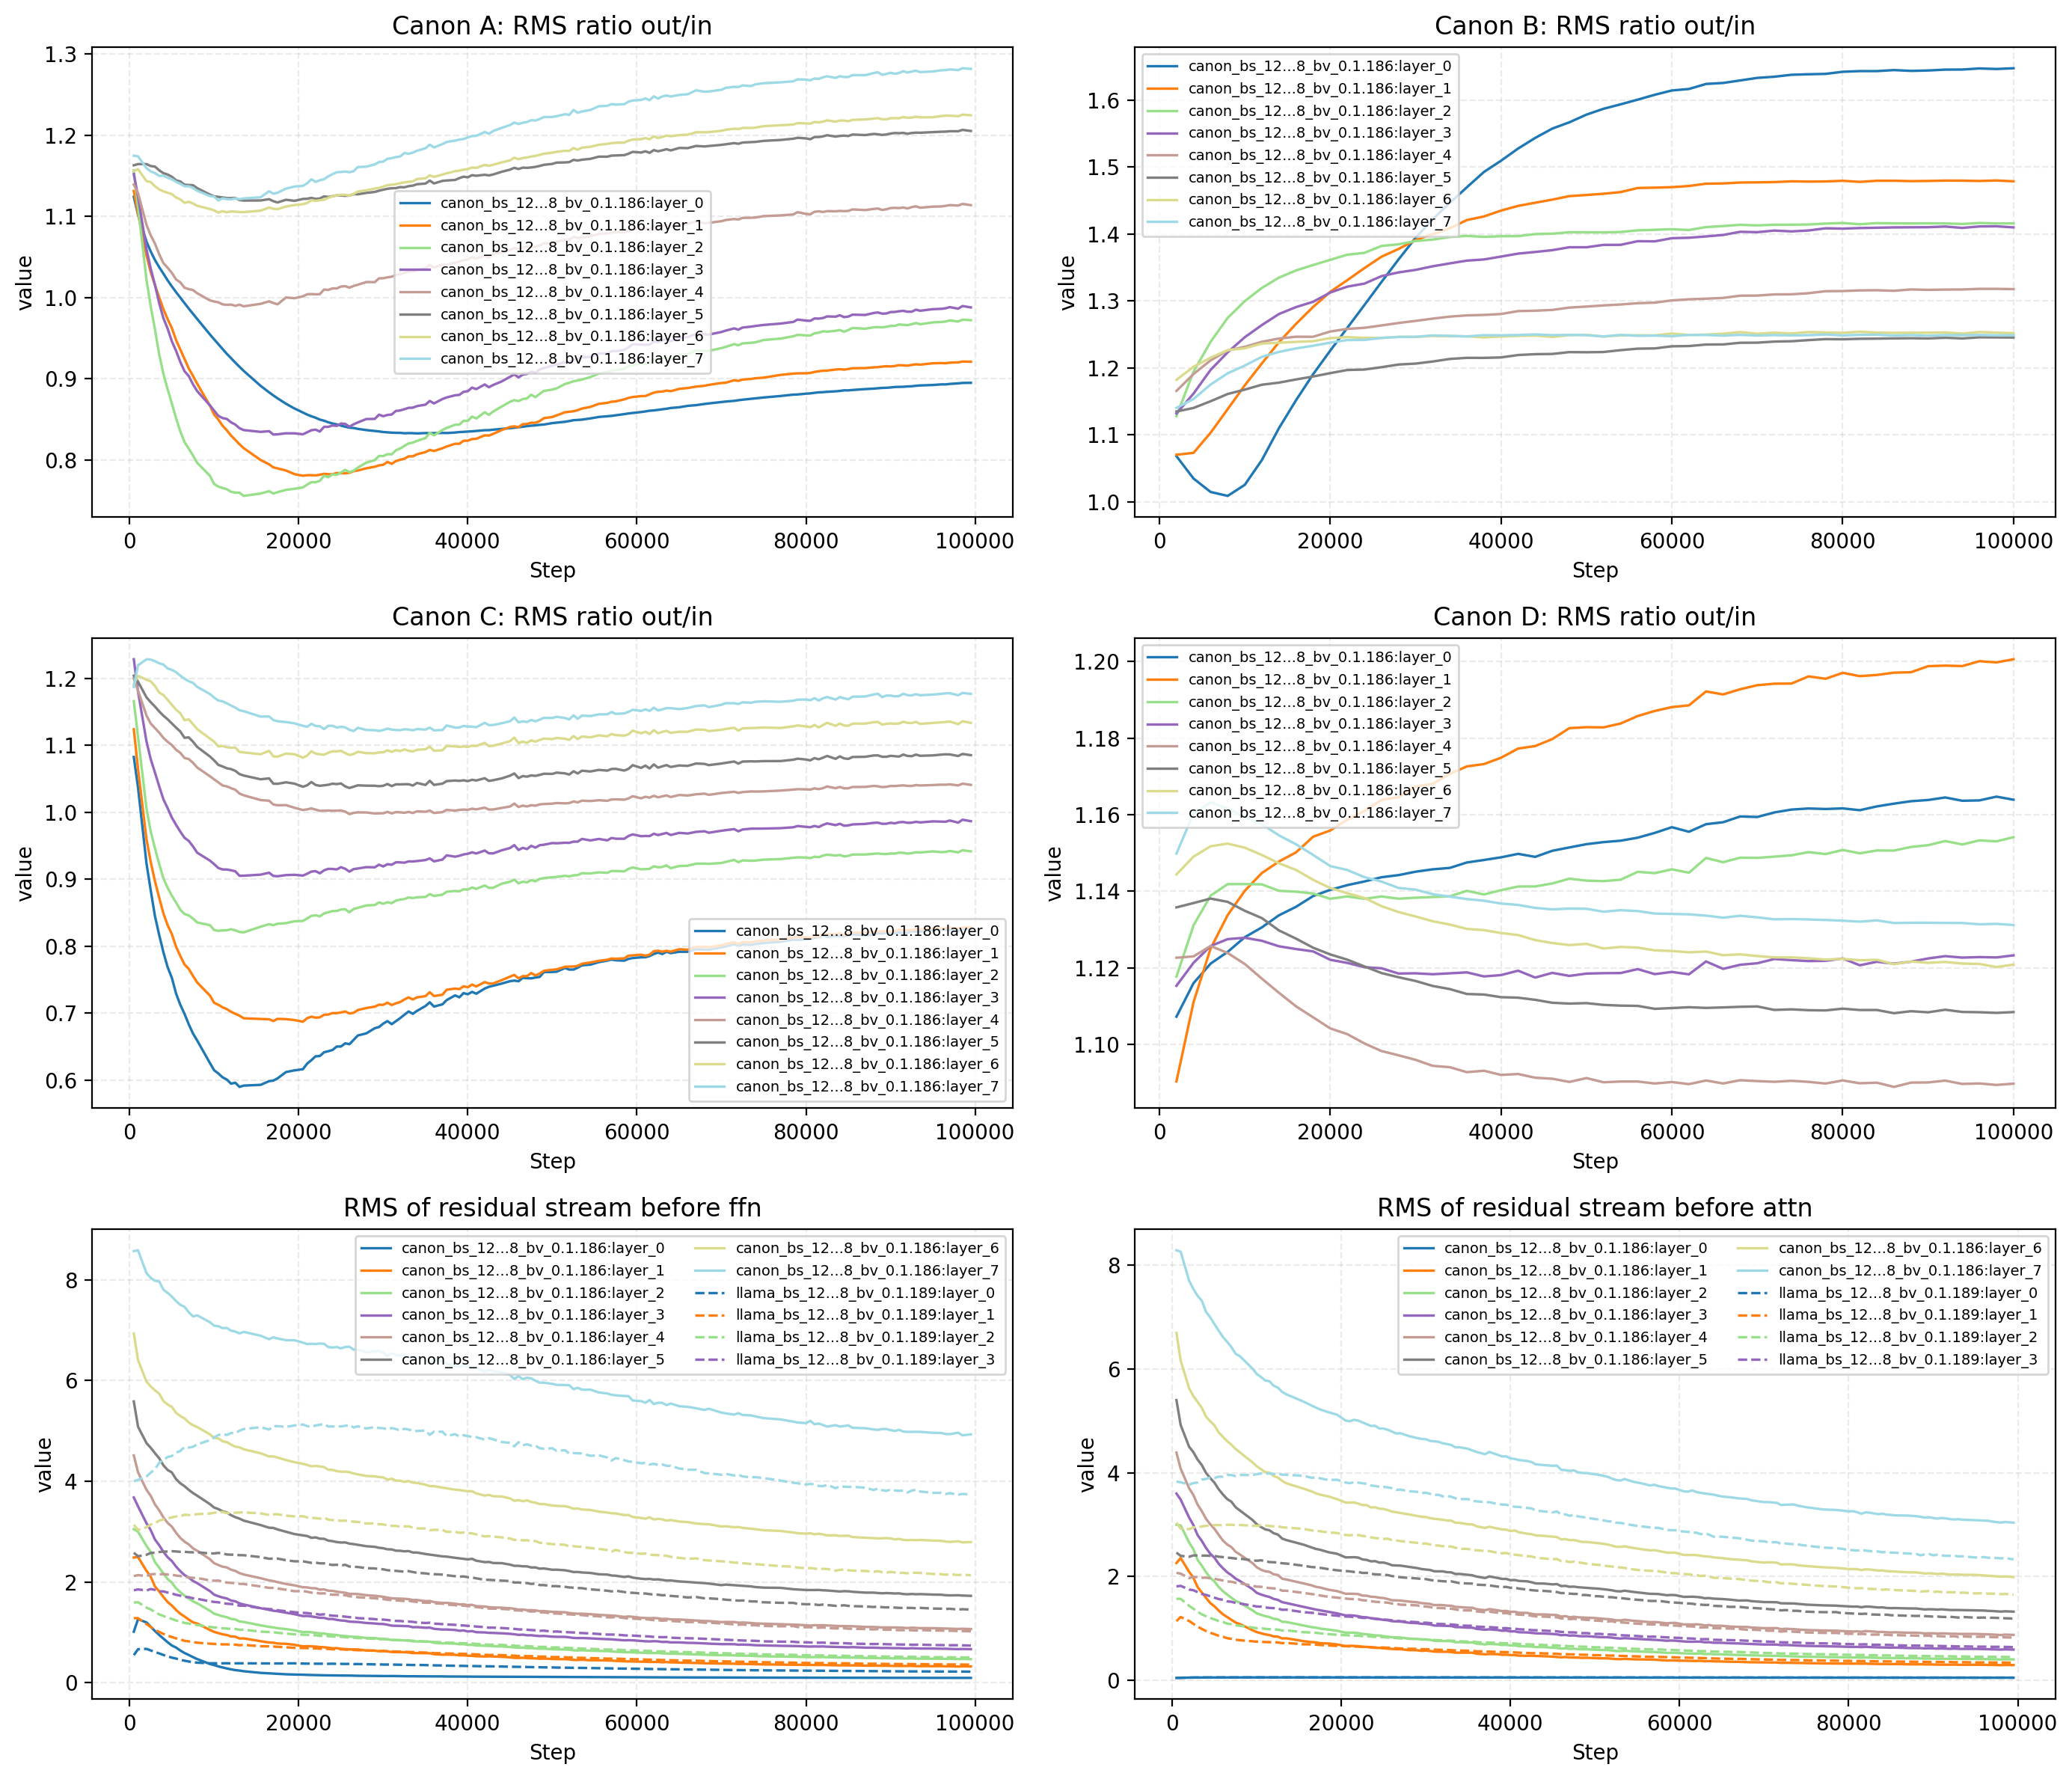
\includegraphics[width=\linewidth]{dynamics_rms_ratio_and_residual.png}
  \caption{RMS ratio of canon output to input (top) and residual stream RMS before
    attention and FFN sublayers (bottom). Canon upscales representations, especially in
    deeper layers.}
  \label{fig:rms_ratio}
\end{figure}

Figure~\ref{fig:rms_ratio} shows the ratio of the output RMS to the input RMS for each
canon type. All canon types amplify the magnitude of representations (ratio $> 1$). The
effect is strongest in deeper layers (closer to the LM head), particularly for types A
and C. This depth-dependent amplification may explain why Canon gains advantage over the
Llama baseline later in training: as the residual stream grows at depth, the canon
contribution compounds.

\subsubsection{Gradient Uniformity}

\begin{figure}[h]
  \centering
  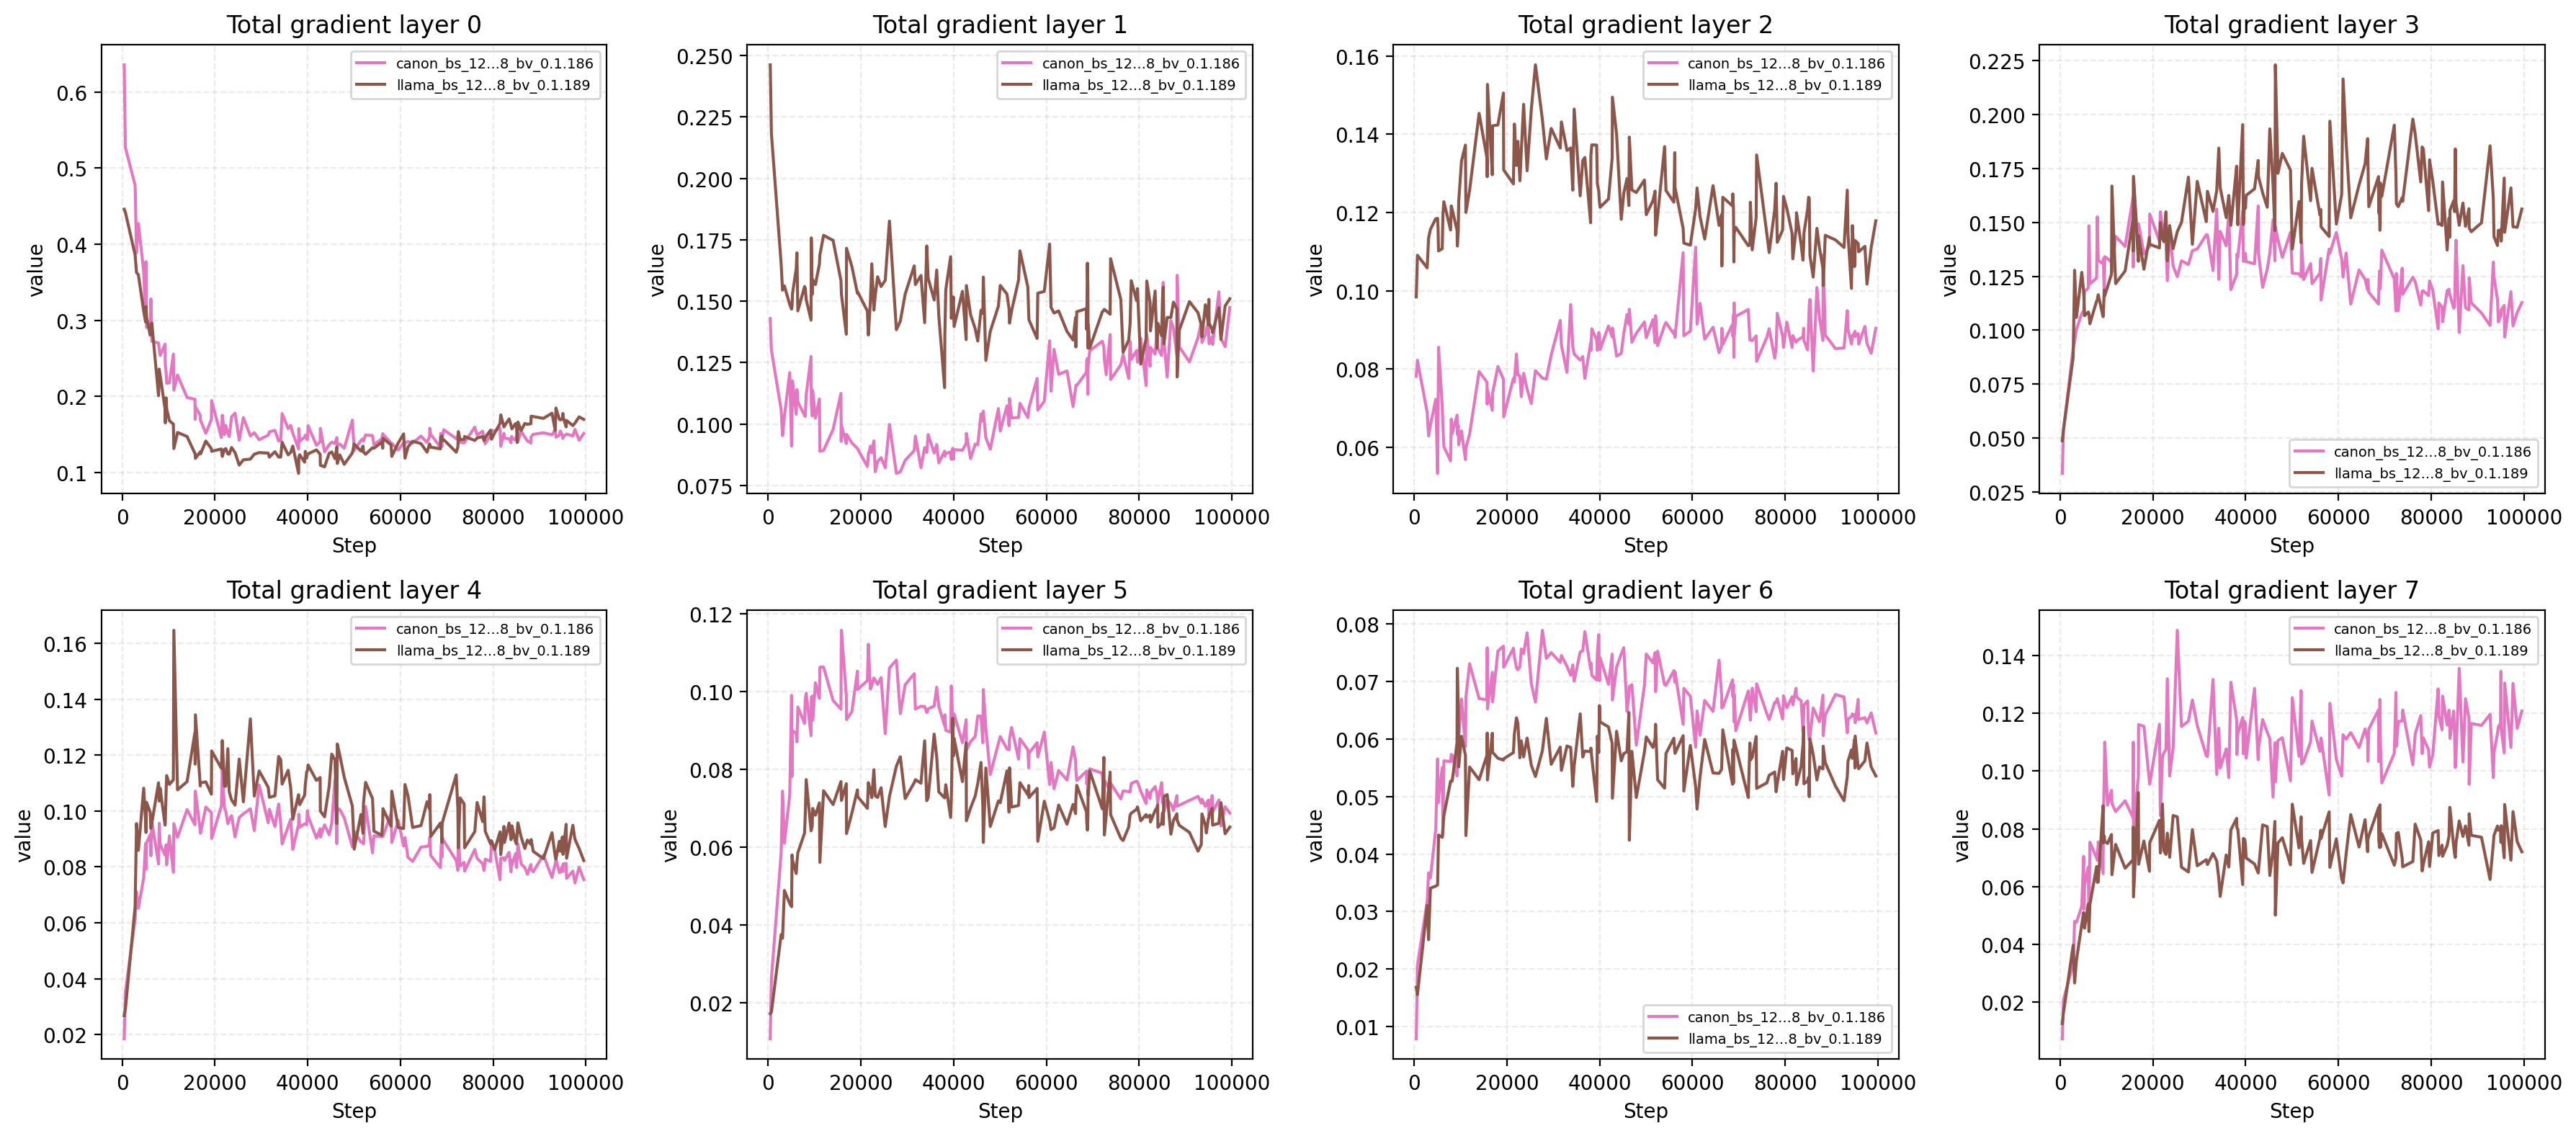
\includegraphics[width=\linewidth]{dynamics_grad_contrib.png}
  \caption{Per-layer gradient contribution magnitudes for Canon and Llama mid-training.
    The Llama baseline shows a steep decline from deep to shallow layers; Canon produces
    a much flatter profile.}
  \label{fig:grad_contrib}
\end{figure}

A well-known challenge in deep network training is gradient imbalance: gradients in early
layers are much smaller than in later layers, slowing learning. Figure~\ref{fig:grad_contrib}
quantifies this for both models. The Llama baseline shows a ratio of approximately
$20/6 \approx 3.3\times$ between the deepest and shallowest layer gradients. Canon
reduces this to approximately $11/8 \approx 1.4\times$, indicating that canon layers
substantially alleviate gradient vanishing in early layers.

\subsubsection{Outlier Features}

\begin{figure}[h]
  \centering
  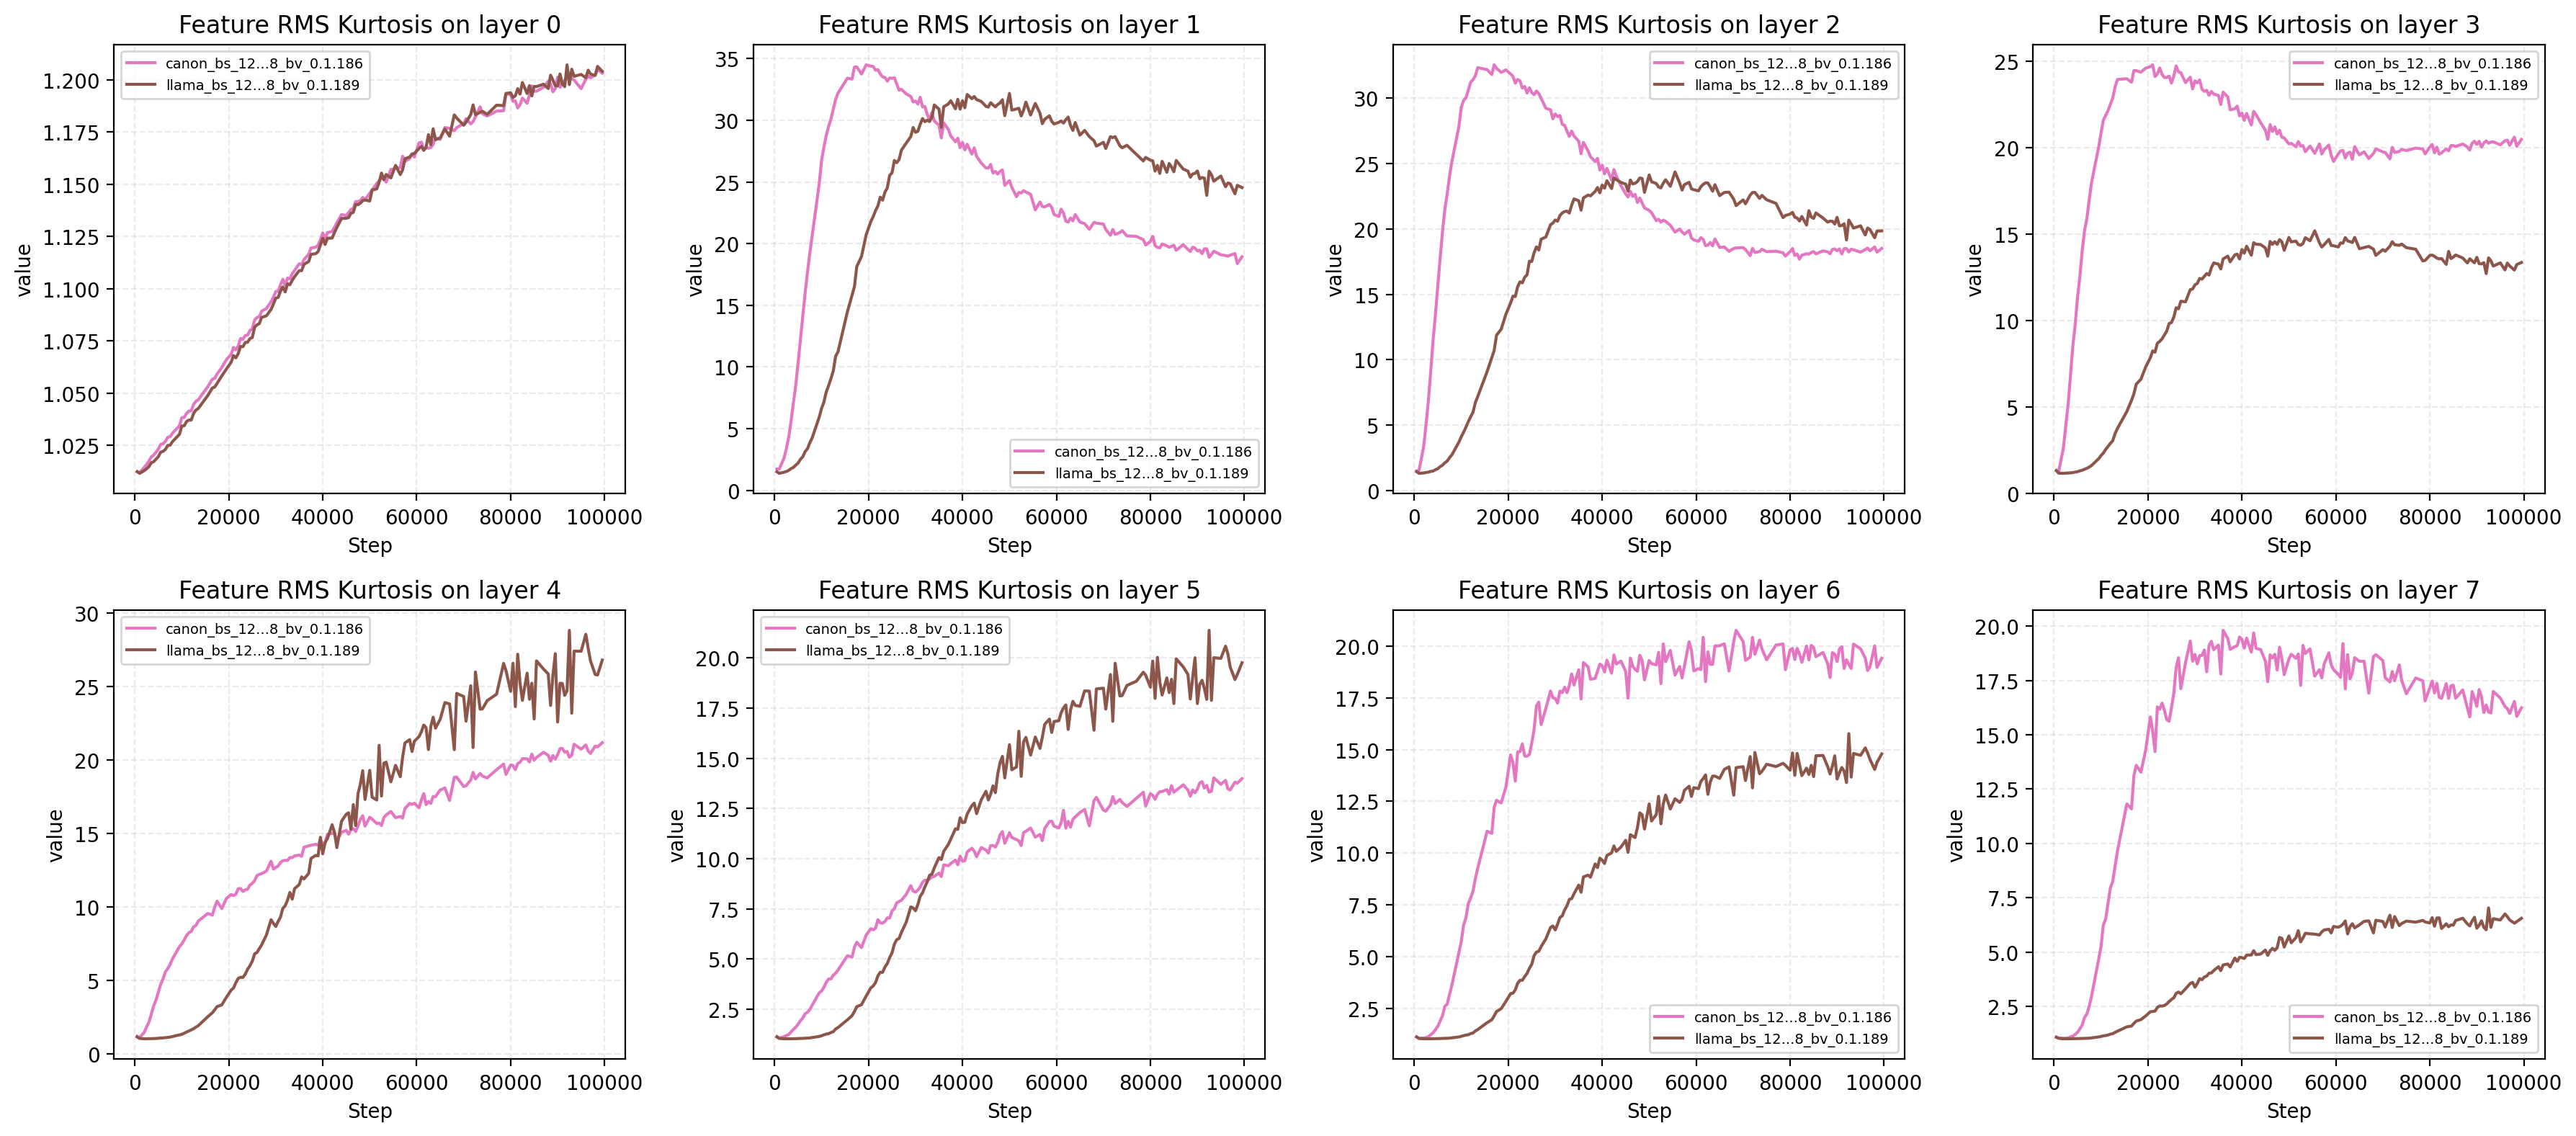
\includegraphics[width=\linewidth]{dynamics_outlier_features_kurtosis.png}
  \caption{Activation kurtosis per layer for Canon and Llama. High kurtosis indicates
    outlier features. Canon greatly reduces kurtosis in all layers except layer 0.}
  \label{fig:kurtosis}
\end{figure}

Outlier features (activations with extreme values) are a known source of training
instability. Figure~\ref{fig:kurtosis} shows activation kurtosis per layer, where high
kurtosis signals the presence of outlier features. Canon dramatically reduces kurtosis
across all layers compared to the Llama baseline, with the notable exception of layer 0,
which retains elevated kurtosis in both models.

\subsubsection{Cosine Similarity Between Canon Output and Input}

\begin{figure}[h]
  \centering
  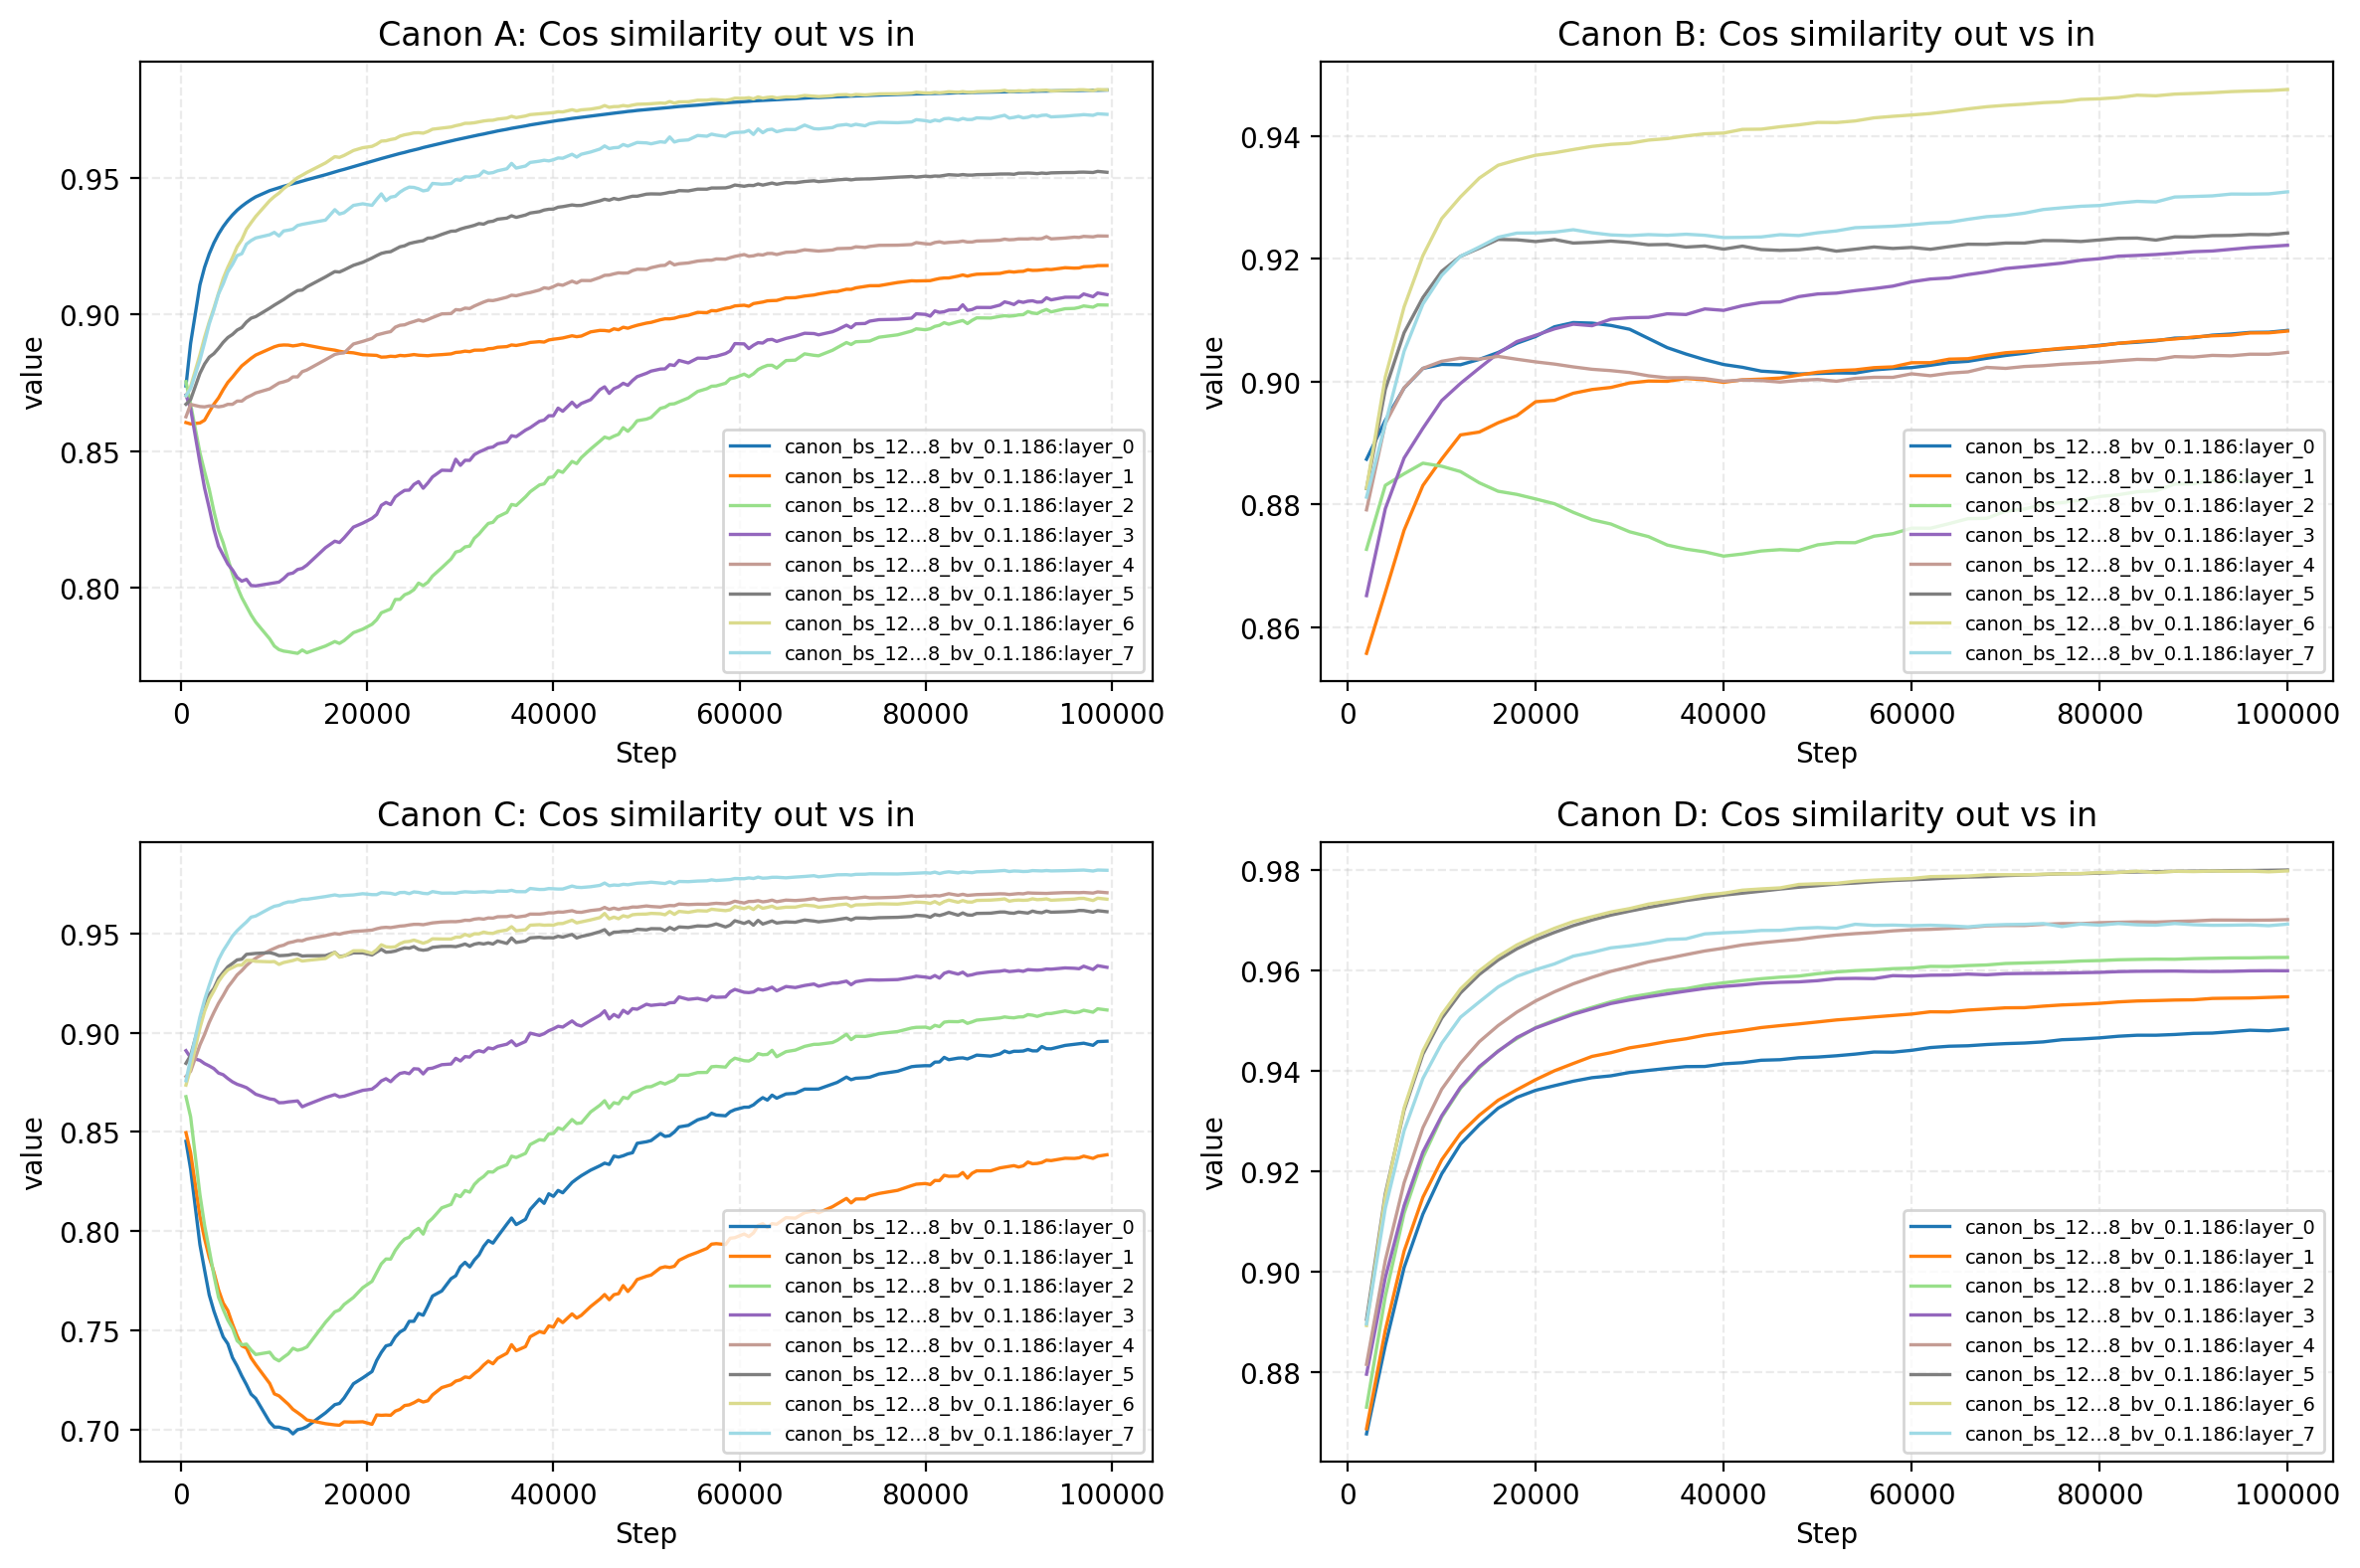
\includegraphics[width=0.7\linewidth]{dynamics_canon_cos_similarity.png}
  \caption{Cosine similarity between the canon output and its input for types A, B, C, D
    across layers. Lower similarity indicates stronger mixing. Canon types A and C mix
    more in early layers; all types converge toward identity-like behavior in deeper
    layers.}
  \label{fig:cos_sim}
\end{figure}

Figure~\ref{fig:cos_sim} measures the cosine similarity between a canon layer's output
and its input across training. A similarity close to 1 indicates the canon is acting as a
near-identity (residual) transformation. Deeper layers show higher cosine similarity for
all canon types, meaning the convolution contributes less mixing as depth increases. Canon
types A and C exhibit stronger mixing (lower similarity) in the first layers, which is
consistent with the representation scaling results showing that A and C have greater
depth-dependent amplification.

\begin{thebibliography}{9}
\bibitem{allen_zhu_physics4}
  Z.\ Allen-Zhu and Y.\ Li.
  \emph{Physics of Language Models: Part 4.1 --- Learning Knowledge
  and Reasoning Skills}.
  arXiv preprint, 2023.

\bibitem{power2022grokking}
  A.\ Power, Y.\ Burda, H.\ Edwards, I.\ Babuschkin, and V.\ Misra.
  \emph{Grokking: Generalization Beyond Overfitting on Small Algorithmic Datasets}.
  arXiv:2201.02177, 2022.
\end{thebibliography}

\end{document}
